\documentclass[11pt,a4paper]{article}
\usepackage[margin=25mm]{geometry}
\usepackage[T1]{fontenc}
\usepackage[utf8]{inputenc}
\usepackage{lmodern,amsmath,amssymb,booktabs,longtable,array,graphicx,calc}
\usepackage{xurl}
\usepackage[round]{natbib}
\usepackage[colorlinks=true,allcolors=blue]{hyperref}
\usepackage{bookmark}
\usepackage{caption}
\captionsetup{font=small,labelfont=bf}
\setlength{\emergencystretch}{3em}
\providecommand{\tightlist}{\setlength{\itemsep}{0pt}\setlength{\parskip}{0pt}}
\providecommand{\pandocbounded}[1]{#1}
\title{Unequal Job Opportunities and Well-Being Inequality: A Latent-Jobs Structural Decomposition}
\author{Hisham Haydar\\University of Luxembourg and LISER}
\date{Build: 09 September 2026\\Discussion draft; intended circulation 10 September 2026}
\begin{document}
\maketitle
\begin{abstract}
Two people who work the same hours for the same pay may be very differently placed: one chose that job from many, the other took the only one available. Income comparisons cannot separate these cases, and the difference matters for how unequal we judge well-being to be.

We estimate a latent-jobs model of labour supply on French single-adult and couple households, in which preferences and a household-specific distribution of available jobs are identified jointly from one likelihood, with every job priced through the tax-benefit system. We then evaluate well-being with a responsibility-side money metric: the uniform pay, offered across the jobs a household can reach, that reproduces the prospect it actually faces.

We find, first, that the utility scale is identified rather than assumed. Fixing the shock scale and the consumption curvature and estimating the consumption weight instead yields 2.03873 for singles and 2.10172 for couples, improving the likelihood by 23.7526 and 15.659 log-points and the population fit from 0.01523 to 0.01304 for singles and 0.01385 to 0.013595 for couples. The money metric is therefore expressed on an estimated scale, not a normalized one.

Second, the behavioural account requires the opportunity distribution: a re-estimated common-opportunity benchmark on the same corrected sample is worse by 141.64 log-points, and the difference is concentrated in exactly the margins the opportunity block governs.

Third, the welfare object is not the theoretical measure but its stochastic, ex-ante extension, and we establish the relationship rather than assuming it. In particular the reference neutralises pay in the utility index while a residual pay channel survives through the opportunity distribution, so the extension does not inherit independence of pay.

Fourth, the decomposition itself. Among single adults, job access and earning opportunities together account for 55.92 per cent of measured inequality in the metric — job access alone 49.16 per cent — against 9.88 per cent for preferences and 34.20 for household resources and needs. Among couples the ordering is different: earning opportunities and resources with household composition dominate, at 35.72 and 51.20 per cent against 8.23 for access. The attribution is exhaustive and the identity is verified rather than imposed. **[AWAITING PARAMETER INTERVALS ON THESE SHARES]**
\end{abstract}

\emph{Status note, stated once. The corrected positive estimation and the corrected welfare decomposition are both complete for singles and couples, and both are what this document reports. Three welfare items are not complete: the cluster-robust parameter intervals on the headline shares, the reconciliation of the bridge statistics between the two welfare measures, and the couples suballocation of resources against household composition. Each is named where it bears. Where a magnitude is unavailable on the corrected frame it is absent, never replaced by a historical value, and the nested resources and needs percentages of earlier drafts are withdrawn rather than relabelled as current.}

\section{Introduction}\label{introduction}

\subsection{The economic question}\label{the-economic-question}

Low earnings can describe someone who prefers more leisure, someone who cannot obtain a well-paid job, or someone whose family resources allow a different work choice. These explanations are observationally entangled but economically different. Income inequality records their combined outcome. It does not tell us how unequal access to employment, hours packages and wage offers affects well-being once people value leisure differently.

The question is how much inequality in well-being is associated with differences in accessible job opportunities, once preferences, resources and household needs are treated explicitly. Answering it requires both a behavioural model and a normative rule for comparing individuals whose opportunities and preferences differ. The behavioural half is a random-utility, random-opportunity model: households choose among job packages, and both their preferences and the relative intensity of the packages available to them enter the distribution of observed choices. Neither object is observed as a complete schedule. The normative half is settled next, before any formula is selected.

\subsubsection{The normative stance, stated before the formula}\label{the-normative-stance-stated-before-the-formula}

Comparing well-being across people with different labour-market prospects requires a decision about which circumstances should enter the comparison itself. We use an \emph{own-opportunity reference}: the monetary benchmark is constructed from the jobs an individual can take, while their actual pay is neutralised in the equal-consumption reference. This separates the valuation of an attained situation from an assumption that everyone faces the same feasible jobs. We then ask how differences in labour-market opportunities, preferences, resources and household needs contribute to inequality under that stated criterion.

The principle is the own-set equal-consumption equivalent of the companion theory project \citep{haydarmaniquet}. Writing \(A_i\) for the jobs available to \(i\) and \(z_i\) for the attained situation, the reference level \(W^1_i\) solves

\[u_i(z_i)=\max_{j\in A_i} u_i(W^1_i,j).\]

The monetary argument is an equivalent consumption amount, so the measure is already money-metric: there is no second, arbitrary conversion from an otherwise complete non-monetary index into euros.

\begin{figure}
\centering
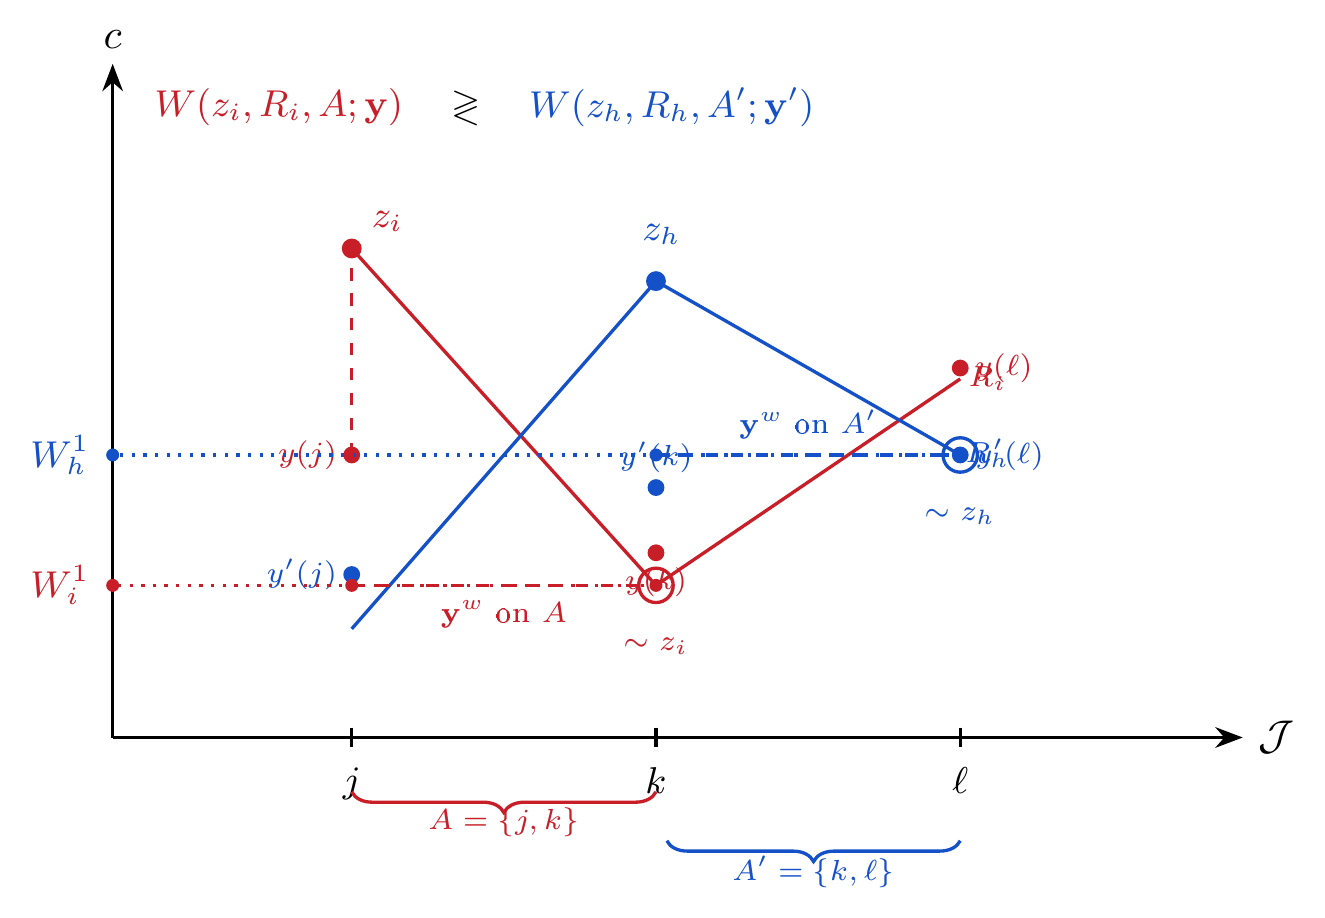
\includegraphics[width=0.95\linewidth,height=\textheight,keepaspectratio,alt={The own-set equal-consumption reference, adapted with permission from the companion theory project's presentation (Haydar--Maniquet, work in progress). Two individuals with different preferences and different sets of available jobs, A=\textbackslash\{j,k\textbackslash\} and A\^{}\{\textbackslash prime\}=\textbackslash\{k,\textbackslash ell\textbackslash\}, attain the bundles z\_i and z\_h. Holding each individual's own preferences and own set fixed, a single flat consumption level is offered at every job in that set and raised until the best job under that level is exactly indifferent to what the individual actually attains; the level at which this happens, read on the consumption axis, is the monetary equivalent. Pay enters nowhere in the reference, because the level is the same at every job; the individual's own set does enter, because the maximisation runs over it. Which individual is better off is what the measure decides, not an assumption of the diagram. Status: a definition, not an estimate --- no axis is calibrated and nothing here is computed from the data.}]{figures/v3/theory_w1.png}
\caption{The own-set equal-consumption reference, adapted with permission from the companion theory project's presentation (Haydar--Maniquet, work in progress). Two individuals with different preferences and different sets of available jobs, \(A=\{j,k\}\) and \(A^{\prime}=\{k,\ell\}\), attain the bundles \(z_i\) and \(z_h\). Holding each individual's own preferences and own set fixed, a single flat consumption level is offered at every job in that set and raised until the best job under that level is exactly indifferent to what the individual actually attains; the level at which this happens, read on the consumption axis, is the monetary equivalent. Pay enters nowhere in the reference, because the level is the same at every job; the individual's own set does enter, because the maximisation runs over it. Which individual is better off is what the measure decides, not an assumption of the diagram. Status: a definition, not an estimate --- no axis is calibrated and nothing here is computed from the data.}
\end{figure}

\textbf{What this principle is, and what it is not.} The companion project associates this measure with independence of pay and with responsibility for equal pay. It does \emph{not} label it full responsibility, and neither do we. It is a particular own-set, pay-neutral reference --- a mixed compensation/responsibility position, not the fully responsibility-oriented endpoint of the family. Nor does selecting it assert that location, education or estimated preferences are morally chosen. Empirical attribution and moral verdict remain different statements throughout.

\textbf{Why the reference depends on the individual's own opportunity set.} A reference satisfying independence of the ability set compares situations at a fixed attained preference level: if \(z\) and \(z'\) are indifferent for \(i\), the measured level is the same whether the opportunity set is \(A\) or \(A'\). That axiom excludes a \emph{direct} reference-set channel. It does not make such a measure insensitive to opportunities, because restricted access can still lower the attained bundle and therefore the measured level through an \emph{indirect attainment} channel. We accordingly do not argue that those measures are mathematically incapable of reflecting opportunity-driven inequality; that argument would be wrong. Our reason is narrower and is a choice, not a theorem: we want the individual's own opportunities to remain relevant to the reference evaluation itself, and not only to the process that produces the attained outcome. Wherever a measure is compared with ours below, these two channels are named separately.

\textbf{An own-set reference is not a claim that larger menus are better.} For fixed attained utility and preferences, enlarging \(A\) weakly raises \(\max_{j\in A}u_i(m,j)\), so with monotone consumption the amount required to match a given attainment weakly falls. The outcome effect of a changed set can offset or outweigh that reference effect. Measuring attainment relative to one's own opportunities is therefore not the same as assigning intrinsic positive value to menu size, and we claim neither general ranking.

\textbf{One borrowed principle, not a borrowed paper.} We use the definition above and the property just described; we do not re-prove the companion project's family of measures or implement it empirically. The welfare section states precisely how the evaluated object relates to this equation, and does not claim that the theoretical characterisation transfers to it.

Two distinctions organize the paper. First, employment and occupation access are not the same mechanism as the distribution of wages conditional on an occupation. Second, neither is the same as non-labour resources or household needs. The exhaustive non-preference component includes all these circumstances, but only its access and earnings components answer the narrower job-opportunity question. Reporting the entire non-preference share as an opportunity share would misstate the estimand.

The paper measures how explicitly modelling household-specific labour-market opportunities changes cross-sectional inequality in an ex-ante money metric and its attribution across preferences, job access, earnings opportunities, resources and needs. Joint preference--opportunity estimation is inherited from the latent-jobs literature, not invented here. The contribution is this estimand, its French single-adult and couple applications, and the comparison with re-estimated common-opportunity benchmarks.

Both halves of that answer are now available. The behavioural half gives corrected samples, a single converged optimum for each population, fresh clustered inference, and a population-level fit that never uses sampled-menu probabilities. The welfare half gives the decomposition, and the answer to the paper's own question is direct for single adults: \textbf{unequal job opportunities --- job access together with earning opportunities --- account for about 56 per cent of measured well-being inequality among single adults.} Job access alone carries 49.16 per cent of it, earning opportunities 6.76, preferences 9.88, and household resources and needs 34.20. Among couples the composition of the answer changes rather than its exhaustiveness, and the contrast between the two household types is itself one of the findings.

What is not reported is narrower, and is named at each point where it bears: the parameter intervals on these shares, the reconciliation of the bridge statistics between the two welfare measures, and the couples suballocation of resources against household composition. No causal effect of geography is claimed anywhere, and no share is pooled across household types.

\section{Related literature}\label{related-literature}

\subsection{Related literature and the exact contribution}\label{related-literature-and-the-exact-contribution}

\subsubsection{Labour supply as choice among latent jobs}\label{labour-supply-as-choice-among-latent-jobs}

The structural labour-supply literature supplies the behavioural machinery needed to take non-linear taxes and heterogeneous preferences seriously. In a standard discrete-hours application, the analyst evaluates a set of hours points, uses a tax-benefit calculator to price them, and estimates preferences from observed choices. That representation is useful but does not by itself distinguish a low probability of choosing an hours package because it is unattractive from a low probability because it is rarely offered. The latent-jobs approach makes this distinction explicit. Jobs can differ in remuneration and working time as well as unobserved attributes; a structural opportunity measure describes their relative intensity.

Dagsvik and Strøm study sectoral labour supply with choice restrictions and flexible functional forms \citep[model exposition]{dagsvikstrom2006}. Sector choice matters because jobs in different sectors need not offer the same hours and earnings opportunities. Their framework is an antecedent for treating the empirical distribution of work as the product of systematic utility and an opportunity component, rather than as a direct image of tastes. What is estimated is a behavioural job-choice model, with restrictions on the functions that describe utility and sectoral opportunities. The relevant inheritance is the discipline of specifying both functions, their domains and their identifying restrictions. It is not permission to import every exclusion, shock process or normalization from their model into ours.

This distinction is especially important at an hours peak. If utility is left sufficiently unrestricted, an observed concentration of hours need not uniquely reveal employer restrictions. Our placement of narrow hours bands in the opportunity function, together with a smooth leisure utility, is a maintained identifying restriction. The separate role of labour-market shifters relies on their exclusion from preferences conditional on the other regressors. The restrictions can be economically motivated by working-time institutions, but the histogram alone does not prove them. Dagsvik and Jia make unobserved heterogeneity and identification central to the latent-jobs formulation \citep{dagsvikjia2016}. Their contribution cautions against interpreting a well-fitting product of preferences and opportunities as a nonparametric recovery of each factor. Our application uses observed preference shifters and a restricted opportunity parameterization; it does not estimate the full persistent unobserved-heterogeneity structure considered in that literature. Failed recovery in a tested extension would not prove that such heterogeneity is absent in France.

More specifically, Dagsvik--Strøm's identification discussion separates the consumption component and conditional wage-offer distribution from the harder leisure/opportunity split. The leisure factor and offered-hours factor appear as a product; separating them requires additional functional restrictions. Their application attributes part-time and full-time clustering to institutional or technological restrictions under that parameterization. It does not establish that arbitrary preferences could never generate clustering. Their empirical random effect also qualifies the independence-of-irrelevant-alternatives assumption: it is conditional on that effect, not an unconditional statement about all households \citep[identification discussion and empirical specification]{dagsvikstrom2006}. We inherit the need to declare the separation restriction, not their entire stochastic specification.

Capéau, Decoster and Dekkers provide the closest applied RURO comparison {[}\citet{capeau2016}, sections on opportunities, preferences and estimation; opportunity-process appendix{]}. They study job choice in Belgium and estimate preferences and opportunities jointly. Their exposition develops the intensity of job offers, the utility attached to jobs, the resulting choice probability and the likelihood, rather than treating offer restrictions as a post-estimation adjustment. Their explicit opportunity-process foundation explains why unobserved jobs may enter a probability model without their complete menus being observed. We inherit joint estimation and the need to distinguish opportunity intensity from choice probability. We do not claim to originate either step.

The distinguishing restrictions again do essential work. Restrictions on the job intensity and utility functions, together with excluded opportunity shifters, separate components that choices alone identify only jointly. Our French model uses employment and occupation access, banded hours and occupation-conditional wage distributions with a household tax-benefit map. It reports single-adult and joint couple applications, then asks about cross-sectional inequality in an ex-ante monetary level and its grouped attribution. Those additions change the object of evaluation and the empirical organization. They do not establish that our application is the first to combine random opportunities with heterogeneous tastes. Nor does the Poisson-process foundation in Capéau and coauthors establish that this code implements that foundation: here the mixed-measure choice density is explicitly maintained as a reduced structural representation.

Capéau and coauthors explicitly assume the wage-offer distribution is independent of offered hours in the identifying argument. They also exclude a group-specific unemployment rate from preferences while allowing it to shift job availability. Their identification subsection explains that the utility and offered-hours factors are not separately recovered nonparametrically without further restrictions. These are concrete antecedents of our conditional wage/hours factorization, labour-market exclusion and smooth-preference/banded-opportunity distinction. Their Belgian application already includes single women, single men and couples. Our inclusion of both household types is therefore not a novelty claim; the change is the French opportunity-sensitive level-inequality estimand and attribution, subject to its own restrictions \citep[identification and empirical-application subsections]{capeau2016}.

\subsubsection{Constrained household choice and welfare already belong together}\label{constrained-household-choice-and-welfare-already-belong-together}

Aaberge, Colombino and Strøm study Italian tax-transfer reforms with an estimated model of partners' simultaneous labour-supply decisions and hours restrictions \citep[section 2 and Appendix A]{aaberge2004}. They compare alternatives including a flat tax, a negative income tax and a workfare arrangement, allowing behavioural responses to alter both resources and their distribution. Their budget maps combine spouses' gross earnings and other income under non-linear tax-transfer rules. This is direct prior work combining joint choice, restricted hours and welfare, not a separate literature that stops before welfare evaluation.

Their monetary evaluation uses a reference household, choice set and tax system to translate attained utility into equivalent income; differences across tax systems assess reform gains. We inherit the lesson that behavioural and distributional evaluation must be linked and that the reference must be stated. Our reference instead flattens disposable consumption across alternatives while retaining the specified state's non-consumption utility and opportunity weights. Our main empirical object is a cross-sectional distribution of levels, not the compensating gain from replacing a tax schedule. These differences are substantive: one cannot transfer their rankings, reform gains or normative reference to our measure merely because both are called equivalent income.

The couple application consequently belongs in the core of the present paper. Jointly pricing two earnings streams under a shared household budget is not equivalent to fitting two independent single-person decisions. Even when the deterministic leisure terms are additive, the non-linear household budget couples their choices. The maintained absence of a direct cross-leisure interaction is a restriction within a joint model, not evidence that the decisions are independent. Our narrower contribution is the opportunity-sensitive cross-sectional welfare attribution, not the discovery that joint labour supply, hours restrictions and welfare can be analysed together.

\subsubsection{Heterogeneous preferences and interpersonal welfare comparison}\label{heterogeneous-preferences-and-interpersonal-welfare-comparison}

Decoster and Haan ask how ethical choices about preference heterogeneity change empirical welfare orderings and the evaluation of a tax reform {[}\citet{decosterhaan2015}; original working-paper version, printed pp.~2--5 and section 2{]}. Their application estimates a discrete-choice model of female labour supply in German couples, holding husbands' labour supply fixed. It uses the estimated preference heterogeneity to compare monetary welfare orderings. This is different from our joint couple choice model, but it confronts the same normative difficulty: equal incomes or common monetary units do not resolve interpersonal comparisons when indifference curves differ.

Their preference-respecting metrics increase when an individual reaches a higher indifference curve of her own preferences. A reference-preference ordering instead removes preference heterogeneity at the evaluative stage. Those are different ethical operations, even when both begin with the same estimated behavioural model. Their wage and rent metrics expose different choices about which circumstances are neutralized and how industrious or work-averse individuals are treated. No single ethical rule follows merely from calling a quantity a money metric. The working-paper discussion explicitly distinguishes retaining preferences in the ordering from replacing them with a planner's common preference ordering.

Their comparison gives priority to preference-respecting evaluation and restricts interpersonal comparisons through nested equivalent sets. The wage criterion indexes the household's own indifference curve by a hypothetical net wage with no unearned-income intercept; the reference-wage class instead fixes a common net wage and varies the unearned-income intercept. The rent criterion is the zero-reference-wage case. Thus the reference removes actual wage and non-labour-income circumstances from the comparison setting while preserving the individual's own preference ordering. Their normative discussion distinguishes compensation for circumstances from liberal reward for preference-related differences: the rent reference offers stronger protection to work-averse individuals than the wage reference. Their empirical preference estimates also exploit tax-schedule variation across years, not solely cross-sectional functional form \citep[original working-paper version, printed pp.~7--11]{decosterhaan2015}. Our single-policy-year application does not inherit that source of identifying variation. Nor is our integration over a reference opportunity distribution equivalent to maximizing over their nested deterministic budget sets.

Our baseline preserves the household's own non-consumption utility and opportunity weights in both attained and reference ex-ante value. Holding that reference fixed, increasing attained value increases the equivalent income. This is the limited, precise sense in which the mapping respects the household's estimated evaluation. It is not a claim that our stochastic set-valued reference satisfies every axiom attached to Decoster--Haan's deterministic bundle metrics. In particular, because the opportunity distribution enters both sides, changes in the menu cannot be assessed by holding the reference curve silently fixed. The preference-equalization counterfactual is a separate exercise: it changes preference shifters in attained value and in the reference map. It should not be described as a baseline measure that already purges all preference differences.

The companion Haydar--Maniquet theory project likewise studies jobs and well-being measurement, but its family of reference principles remains distinct \citep{haydarmaniquet}. This application evaluates one specified flat-consumption reference. The illustrative consumption--leisure diagram motivates the ambiguity in observed work; it neither proves an axiomatic characterization of the empirical index nor implements the entire companion theory. The separation matters because reference design is a scientific and ethical choice that behavioural estimation cannot settle on its own.

\subsubsection{Responsibility-sensitive reform effects versus cross-sectional levels}\label{responsibility-sensitive-reform-effects-versus-cross-sectional-levels}

Jacquet, Jia and Thoresen use a job-choice model to compare standard and circumstance-only compensating variation for a Norwegian tax reform \citep[sections 3--5]{jacquet2026}. They distinguish the welfare effect evaluated with individual preferences from a responsibility-sensitive effect computed after replacing preference characteristics by reference values. Their model treats couples as unitary joint decision makers, and its observed and unobserved preference heterogeneity informs the comparison. The object is a welfare change between policy regimes, with a declared treatment of preference-related differences, rather than the distribution of monetary levels under one policy system.

We inherit their insistence that the preference--circumstance distinction must be made explicit in welfare evaluation and that a latent-jobs model is useful for doing so. The empirical question changes here: how much cross-sectional inequality in an ex-ante monetary level is allocated to preferences, access, earnings opportunities, resources and needs? A reform compensating variation and a cross-sectional equivalent-income level have different origins and denominators. Even if their preference-related reform differences were small, that would not establish a small preference contribution to our level inequality. Conversely, our decomposition would not estimate the welfare gains of their reform. Neither comparison should be presented as a numerical validation of the other.

\subsubsection{Distributional attribution and the role of grouping}\label{distributional-attribution-and-the-role-of-grouping}

Shorrocks develops decomposition procedures using the Shapley value to allocate a distributional change across factors \citep{shorrocks2013}. The economic difficulty is that the effect of equalizing one factor depends on which others have already been equalized. Non-linear taxes, consumption utility and household needs make such interactions unavoidable here. Averaging marginal effects across orders produces an exhaustive attribution of the reducible inequality difference without assigning all interactions to the last factor changed. This is an allocation principle, not an identification result or a causal estimator.

The grouped implementation gives the preference versus non-preference distinction priority, then allocates the non-preference component among its mechanisms. The Shapley--Owen--Shorrocks discussion in Audoly and coauthors clarifies this hierarchy \citep{audoly2025}. Grouping is a maintained economic design choice: it ensures that the broad preference--circumstance comparison is not changed solely by subdividing one circumstance into many labels. A flat allocation over all subfactors would generally allocate cross-group interactions differently. It is a legitimate alternative question, not an algebraic error to be repaired by rescaling its contributions.

Together these literatures narrow the contribution. Latent-job estimation, non-linear taxes, joint household choice, preference-sensitive welfare and Shapley allocation all have precedents. What the present exercise adds is the explicit measurement of how household-specific labour-market opportunities change cross-sectional inequality in the implemented ex-ante money metric, separated from resources and needs, with a re-estimated common-opportunity comparison. The empirical magnitude and its sensitivity remain to be established by the corrected results.

\section{Conceptual framework}\label{conceptual-framework}

\subsection{From observed work to the implemented reference}\label{from-observed-work-to-the-implemented-reference}

An observed job is a package of working time, occupation and hourly remuneration. Simulated alternatives are jobs drawn by the analyst to evaluate integrals or a sampled-choice likelihood; they are not a recovered list of the jobs a household actually received. A consumption--leisure picture clarifies why one observed package cannot identify its explanation. The same bundle may be optimal when the household places considerable value on leisure and has broad options, or when a more work-oriented household faces a tighter menu.

\begin{figure}
\centering
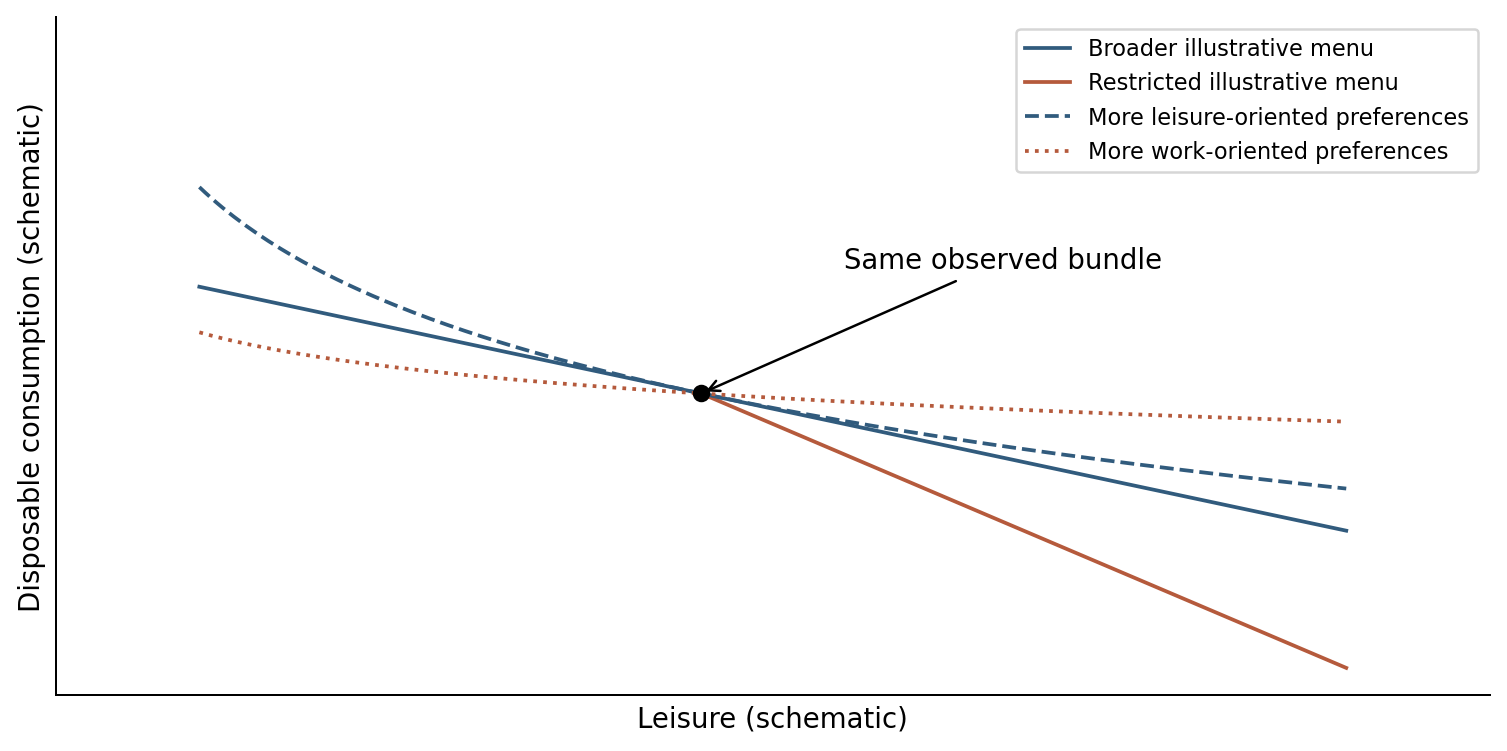
\includegraphics[width=0.95\linewidth,height=\textheight,keepaspectratio,alt={Motivation only: a schematic single-person consumption--leisure ambiguity. Axes have no empirical calibration; menus and preferences are illustrative. The same observed bundle does not identify its explanation. The conceptual distinction is related to Haydar--Maniquet's companion theory paper; no fixed-leisure equivalent-income measure is computed.}]{figures/v3/motivation.png}
\caption{Motivation only: a schematic single-person consumption--leisure ambiguity. Axes have no empirical calibration; menus and preferences are illustrative. The same observed bundle does not identify its explanation. The conceptual distinction is related to Haydar--Maniquet's companion theory paper; no fixed-leisure equivalent-income measure is computed.}
\end{figure}

The figure is motivation, not an empirical estimate or a computation of our money metric. It uses the consumption--leisure distinction discussed by Haydar and Maniquet in the separate companion manuscript, \emph{Jobs and Well-Being Measurement} \citep{haydarmaniquet}. The graphical construction here is new and schematic. We neither reproduce that paper's full family of welfare measures nor claim its axioms characterize the empirical measure below. In particular, no fixed-leisure intersection is labelled as the implemented equivalent income.

The implemented monetary reference instead assigns the same disposable-consumption amount \(m\) to every alternative in the reference opportunity distribution. Let \(L_i(j)\) be all non-consumption utility at job \(j\), \(C_i(j)\) priced monthly disposable consumption, \(\lambda_c\) its positive scaling constant, and \(\widehat g_i\) the normalized opportunity density. Define \(BC\) as the Box--Cox function specified in the model section. The bridge from a monetary amount to ex-ante value is

\[\Phi_i(m)=BC(m/\lambda_c;\theta_c)+\log\!\int \exp\{L_i(j)\}\widehat g_i(j)\,d\nu(j).\]

The equivalent income is the amount for which this curve reaches the attained value \(\log\int\exp\{L_i(j)+BC(C_i(j)/\lambda_c;\theta_c)\}\widehat g_i(j)d\nu(j)\). The reference retains leisure differences across alternatives and, at baseline, the household's own preferences and opportunity distribution. It flattens disposable consumption, not leisure, hourly pay or gross earnings. This distinction is the reason for the second early figure.

\begin{figure}
\centering
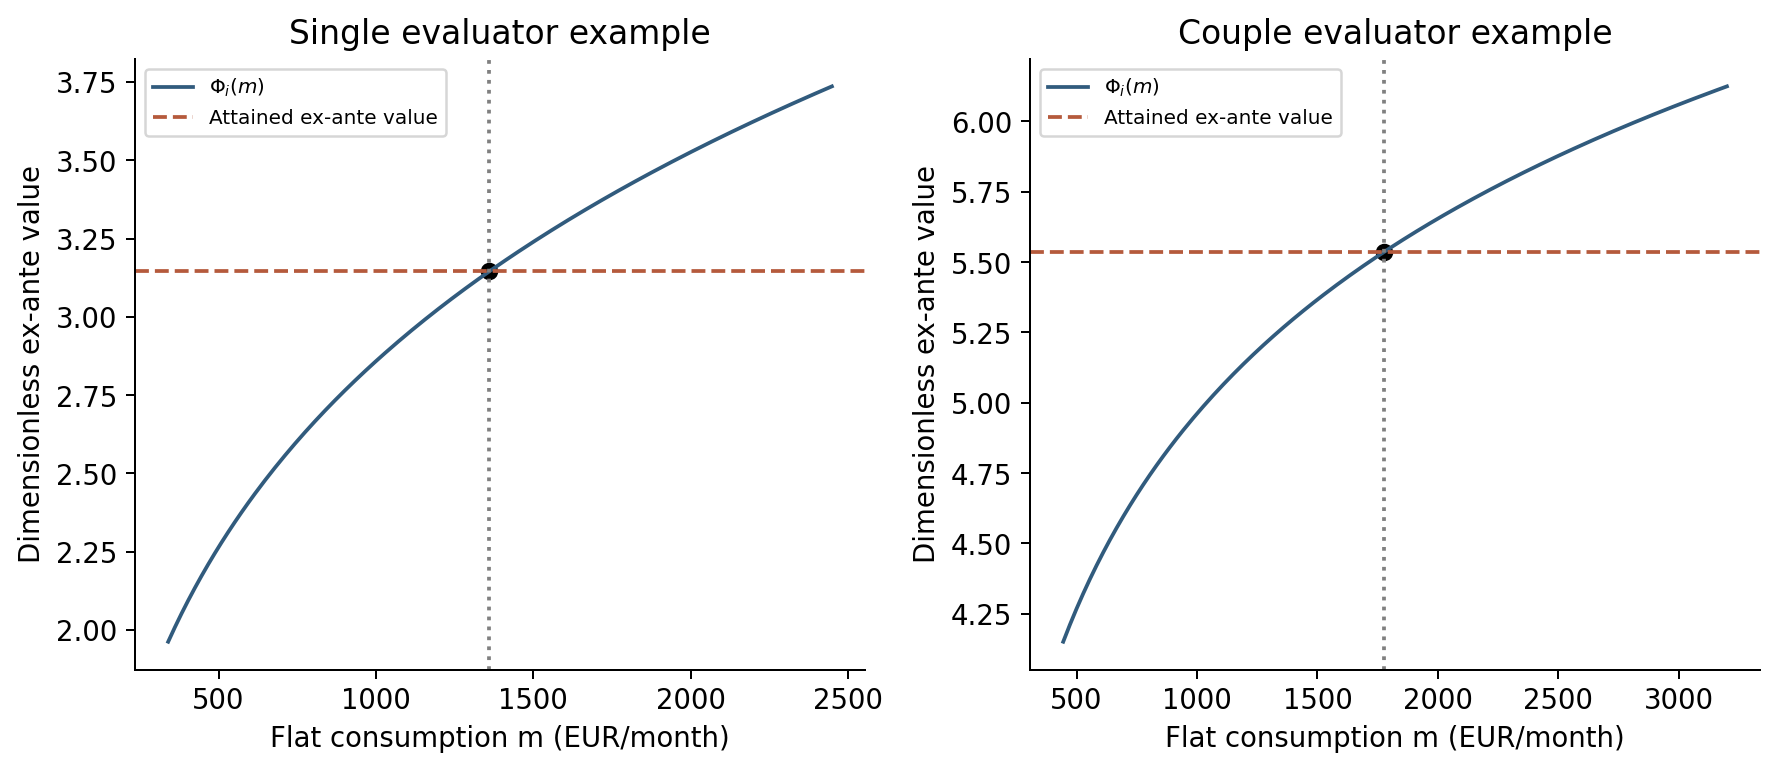
\includegraphics[width=0.95\linewidth,height=\textheight,keepaspectratio,alt={Implemented monetary reference for the anonymous single-adult and couple examples. Horizontal unit: flat monthly disposable consumption in euros; vertical measure: dimensionless ex-ante value. The reference curve meets attained value at equivalent income. Status: current evaluator at historical estimates and priced inputs; not corrected welfare results. Each curve uses its own baseline opportunity distribution and leisure utility.}]{figures/v3/reference_map.png}
\caption{Implemented monetary reference for the anonymous single-adult and couple examples. Horizontal unit: flat monthly disposable consumption in euros; vertical measure: dimensionless ex-ante value. The reference curve meets attained value at equivalent income. Status: current evaluator at historical estimates and priced inputs; not corrected welfare results. Each curve uses its own baseline opportunity distribution and leisure utility.}
\end{figure}

Changing the reference to one fixed leisure bundle would change the question and generally the monetary answer. Expressing both answers in euros would not make them interchangeable. The later welfare section derives the implemented identity and shows its numerical evaluation for a single adult and a couple.

\section{Data and institutional setting}\label{data-and-institutional-setting}

\subsection{French data, timing and institutional setting}\label{french-data-timing-and-institutional-setting}

The application uses the French component of EU-SILC, the European Union Statistics on Income and Living Conditions. Three institutional steps are distinct and are kept distinct here. EU-SILC is collected nationally and harmonised for cross-country comparability by Eurostat, which is the access route for the microdata. That harmonised survey is then transformed into an EUROMOD input file, a separate operation with its own conventions that Eurostat does not itself perform. Finally EUROMOD, the European tax-benefit microsimulation model, applies statutory policy rules to that input to produce simulated disposable resources. The survey supplies the observations; the simulator supplies the budget; neither supplies the other. Simulated disposable resources are not observed consumption expenditure, and this document never calls them that. The input carries 2016 survey collection with a 2015 income-reference year, priced with the French 2015 policy system.

\textbf{Why France, and what the regional dimension supplies.} The application needs harmonised household budgets that can be priced through a validated policy simulator and linked to labour-market conditions measured for the same groups. France supplies all three within one national institutional setting: a large EU-SILC sample, a maintained EUROMOD policy system, and regional labour-force series broken down by education and sex on a classification that can be crosswalked to the survey's regions. The regional dimension therefore contributes \emph{measured heterogeneity in labour-market conditions across groups that face a common tax-benefit system}, which is what identifies differences in access separately from differences in the budget. It supplies nothing more than that. Administrative regions are categorical variables, not a research design: their discreteness does not make them exogenous, does not separate them from commuting and residential sorting, and does not deliver a causal effect of location. We accordingly write of regional labour-market heterogeneity throughout, never of segregated or disconnected regional labour markets, and no estimate below is a causal region effect. Collection, annual income, current hours/status and policy dates are distinct. The input filename does not establish a price deflator, and the tables are not labelled ``real collection-year euros.'' Current-status hours combined with annual income require a mixed-period measurement assumption. The source-to-sample audit identifies that assumption rather than claiming the data observe a complete contemporaneous budget schedule.

EUROMOD is a tax-benefit microsimulation model: it applies policy rules to household inputs to calculate taxes, contributions, benefits and disposable resources \citep{sutherlandfigari2013}. Its chosen-state disposable income is simulated under the policy rules, not observed household consumption expenditure. A counterfactual working job is priced as full-year employment at its weekly hours and gross hourly wage. For spouse \(s\), the actual job operator uses

\[Y_{is}^{\rm reg}=\frac{52}{12}w_{is}\min(h_{is},35),\quad
Y_{is}^{\rm ot}=\frac{52}{12}w_{is}\max(h_{is}-35,0),\quad
Y_{is}=Y_{is}^{\rm reg}+Y_{is}^{\rm ot}.\]

Here \(h\) is hours per week, \(w\) gross euros per hour and \(Y\) gross euros per month. Non-employment sets the alternative's employee earnings and associated job-history inputs accordingly. Equal total earnings with different regular/overtime hours need not produce identical tax inputs. The policy map therefore retains hours and the earnings split, rather than being described as a function of \(wh\) alone.

For a household roster \(\mathcal H_i\), write the corrected target budget as

\[C_i(j)=\mathcal B_\tau\!\left(\{Y_{is}^{\rm reg},Y_{is}^{\rm ot},h_{is}\}_s;r_i,d_i,t_i\right),\]

where \(r_i\) denotes non-labour resources, \(d_i\) composition and other policy-relevant inputs, \(t_i\) the imputed take-up traits, and \(\tau\) the fixed policy system. Disposable resources are aggregated across the complete modelled household using the source's person and allocation semantics. Single-adult consumption sums every resident member's simulated disposable income, on the same rule as couples; the earlier decider-only construction is not used. The retained components satisfy the accounting identity linking disposable income to original income, benefits, taxes and social contributions, with a maximum absolute residual below \(10^{-11}\) euros in both populations.

Resource inputs are heterogeneous objects. Annual cash flows are supplied as monthly equivalents; wealth is a stock; housing costs are expenditure flows; receipt-month variables count months; categorical asset indicators are codes. Employee fringe benefits are non-cash and must not be added to a positive cash-income subtotal as though they were cash. Company cars and imputed housing rent are not childcare or child-unit measures. The field dictionary now resolves the formerly missing unit definitions and these semantic mistakes. Whether alternative-specific work-history counters belong in an independently equalizable resource block remains open, because the job operator overwrites them.

Take-up is an imputation assumption, not a preference estimated from the job-choice likelihood. Revealed cases retain their observed trait; other cases use one seeded household trait per employment state, with separately calibrated singles and couples rates. The pricing workflow must neutralize the simulator's corresponding random take-up step and apply the trait once. The historical positive-consumption floor is not a subsistence estimate. The successor direction treats non-positive disposable consumption as outside the utility domain; its implementation and affected-sample consequences must be established before the dependent results are used.

\subsection{Sample construction for singles and couples}\label{sample-construction-for-singles-and-couples}

The decision unit is a household with one adult decider or a linked opposite-sex couple of deciders. Other residents can affect resources and needs without becoming additional labour-supply decision makers. Couples are not obtained by pairing independent estimates for singles. Both adults must meet the couple eligibility conditions, and the household is the sampling and welfare unit.

The construction starts with the complete household roster, selects the supported household structures, limits each decider's age, excludes current schooling and retirement, disability or survivor-benefit cases, restricts labour-market states, and removes households with an additional employable or earning non-decider. The age field records age, not birth year. The last historical step screens wages and projects hours onto the old model domain. These are selection and measurement operations, not harmless changes of labels. Some employed records without observed employee earnings retain imputed wage inputs: the delivered wage input is not uniformly an observed wage. The following counts describe the historical priced estimation frames; successor counts will be regenerated from the corrected source-to-sample output rather than preserved as targets.

Historical sample flow. Population: French eligible single-adult and linked couple households; unit: unweighted households remaining after each screen; measure: retained count; reference: collection-year input and old observation/support rules; status: observed-input construction, not corrected successor counts.

{ % do not increment counter
\small\setlength{\tabcolsep}{3pt}\begin{longtable}[]{@{}>{\raggedright\arraybackslash}p{0.4800\linewidth}>{\raggedright\arraybackslash}p{0.2150\linewidth}>{\raggedright\arraybackslash}p{0.2150\linewidth}@{}}
\toprule\noalign{}
Screen & Singles & Couples \\
\midrule\noalign{}
\endhead
\bottomrule\noalign{}
\endlastfoot
one- or two-adult households (composition screen) & 4,038 & 5,965 \\
every adult aged 20 to 60 & 2,131 & 3,662 \\
no adult still in education & 2,036 & 3,521 \\
no old-age, disability or survivor pension receipt & 1,755 & 3,218 \\
labour status in scope & 1,598 & 2,412 \\
no other employable or earning member & 1,564 & 2,323 \\
Historical wage screen and hours projection & 1,555 & 2,275 \\
\end{longtable}
}

The historical minimum positive employed hours is 6 for singles, 9 for couple men and 6 for couple women. These observed minima do not change the lower endpoint of a continuous structural hours support. The rule adopted is exclusion of the decision unit: employed hours outside \([5,70]\) per week fall outside the support the continuous hours density is defined on, and five single-adult and twenty-four couple households are dropped on that ground. No record is recoded as non-employed and none is imputed to a mode. Households whose occupation is unrecorded are excluded on the same principle, occupation being a coordinate of the alternative rather than an optional attribute, and three single-adult households with non-positive observed consumption are excluded and listed for inspection rather than repaired.

ISCO means the International Standard Classification of Occupations. The application aggregates its major groups into four project categories, which are aggregates chosen for this model and not official ILO task categories: major groups 6--9 (skilled agricultural work, craft and trades, plant and machine operators, and elementary occupations); major group 5 (services and sales); major group 4 (clerical support); and major groups 1--3 (managers, professionals, and technicians and associate professionals). Craft and operator occupations belong to the first category, not to the clerical one. Military occupations do not have a genuine civilian group in this mapping. Their household treatment must follow the corrected sample decision, not modal re-imputation. The population excludes other household structures and self-employment margins not modelled here; its results are not automatically representative of all French adults.

The preference child count is all resident members below the model's age cutoff, not necessarily the decider's parent-linked minors. Parent-linked children, youngest-child measures and the equivalence-scale count are different variables. Their disagreement does not itself establish a coding error. Replacing one by another would change the model and requires a new estimate.

\subsection{Descriptive distributions and what they measure}\label{descriptive-distributions-and-what-they-measure}

Survey weights expand sampled households to their represented population. A household weight is used once per household, not once per member or simulated job. The normalized weights \(\omega_i=d_i^{\rm survey}/\sum_jd_j^{\rm survey}\) sum to one and are used for descriptive distributions, population predictions and inequality. The structural criterion described later is a sum of household log contributions; this is separate from applying survey weights to a population summary.

Historical sample descriptives. Population: retained singles and couple deciders; household-survey-weighted means/fractions/medians; units stated in rows; reference: old constructed employment/hours/wage inputs; status: observed-input summaries, not model predictions or corrected-sample findings.

{ % do not increment counter
\small\setlength{\tabcolsep}{3pt}\begin{longtable}[]{@{}>{\raggedright\arraybackslash}p{0.2500\linewidth}>{\raggedright\arraybackslash}p{0.2200\linewidth}>{\raggedright\arraybackslash}p{0.2200\linewidth}>{\raggedright\arraybackslash}p{0.2200\linewidth}@{}}
\toprule\noalign{}
Measure & Singles & Couple men & Couple women \\
\midrule\noalign{}
\endhead
\bottomrule\noalign{}
\endlastfoot
Mean decider age (years) & 41.0 & 39.8 & 37.8 \\
Employment fraction & 0.871 & 0.924 & 0.897 \\
Mean hours among employed (hours/week) & 37.7 & 41.4 & 36.0 \\
Median wage input among employed (EUR/hour) & 14.07 & 15.44 & 13.54 \\
\end{longtable}
}

The resource distribution uses actual resource inputs, not the distribution of disposable consumption as a proxy. Chosen-state consumption is a simulated policy output, while wage constructions and hours originate in the survey input with the stated observation rules. These distinctions prevent a mechanically persuasive but economically mislabeled comparison.

\begin{figure}
\centering
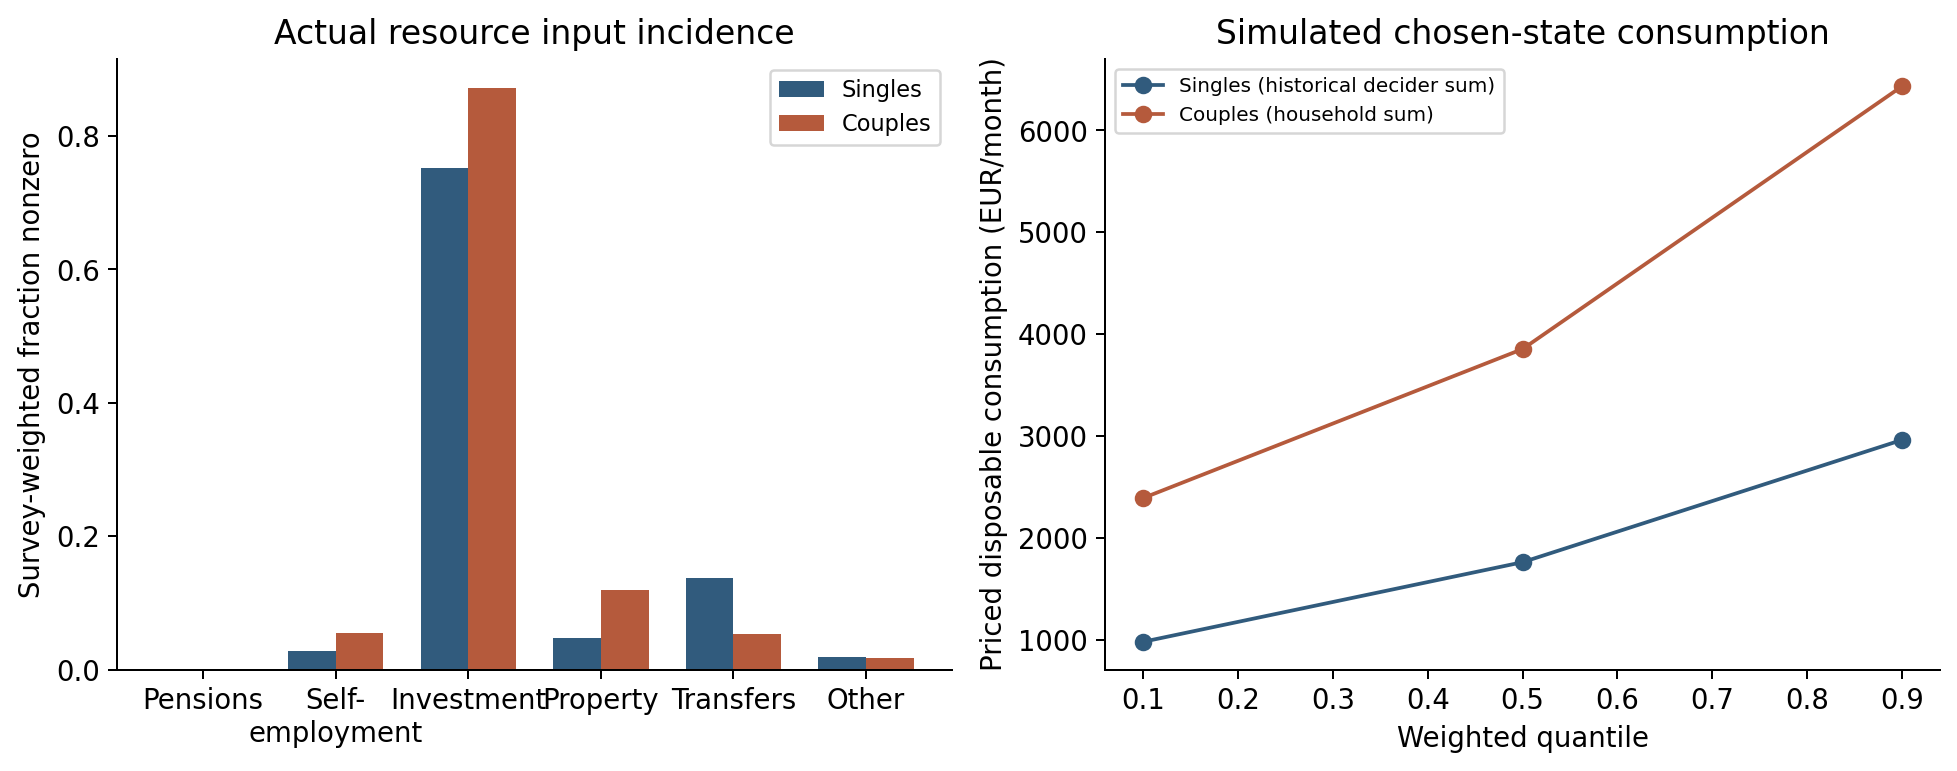
\includegraphics[width=0.95\linewidth,height=\textheight,keepaspectratio,alt={Historical input distributions for retained French singles and couples, using household survey weights. Left: fraction with nonzero actual resource inputs, not consumption proxies. Right: priced chosen-state consumption quantiles, euros/month under the income-reference policy. The singles historical aggregation is decider-based; couples use all-member aggregation. Status: historical source/pricing evidence, not corrected sample or welfare estimates.}]{figures/v3/descriptives.png}
\caption{Historical input distributions for retained French singles and couples, using household survey weights. Left: fraction with nonzero actual resource inputs, not consumption proxies. Right: priced chosen-state consumption quantiles, euros/month under the income-reference policy. The singles historical aggregation is decider-based; couples use all-member aggregation. Status: historical source/pricing evidence, not corrected sample or welfare estimates.}
\end{figure}

The current descriptives reveal the sample and the economic scales used by the historical computation. They do not establish corrected behavioural fit. Singles and couples have different resource pooling and composition; a higher household consumption level for couples is not evidence of higher individual well-being without a needs adjustment and an explicit intra-household interpretation. The corrected sample and all-member budget rebuild may change the distributions, so the figure is marked historical input evidence locally, not only in the version note.

\section{Structural household model and identification}\label{structural-household-model-and-identification}

\subsection{The household model and its maintained assumptions}\label{the-household-model-and-its-maintained-assumptions}

For household \(i\), \(j\) is a single job or a joint pair of jobs. A single non-employed alternative is denoted \(0\); working jobs have occupation \(k\), hours \(h\) and wage \(w\). Let \(T\) be the weekly time endowment and \(\lambda_\ell\) the leisure scale in hours per week. Define dimensionless consumption \(c=C/\lambda_c\) and leisure \(\ell=(T-h)/\lambda_\ell\) on the positive-leisure support. The historical guard \(\max(T-h,1)\) is inactive inside the stated hours domain; it is not authority to expand that domain without checking the leisure interpretation.

\[BC(z;\theta)=\begin{cases}(z^\theta-1)/\theta,&\theta\ne0,\\\log z,&\theta=0,\end{cases}\qquad z>0.\]

For single adults of sex \(s\), deterministic utility is

\[u_i(j)=\omega_{is}BC(\ell_i(j);\theta_{\ell s})+BC(c_i(j);\theta_c),\] \[\omega_{is}=\beta_{\ell0,s}+\beta_{\ell a,s}a_i+\beta_{\ell a2,s}a_i^2+
\mathbf1\{s=f\}\beta_{\ell n,f}n_i.\]

Here \(a_i\) is age centred using the frame's decider-age mean and divided by 10 years; \(n_i\) counts all resident members younger than 20 years. The age square is recomputed after centring and scaling. The child effect is additive in the leisure weight. It is not an exponentiated proportional change in that weight, and the absence of a male child term is a maintained structural zero, not a precise estimated zero.

For a couple, the actual maintained specification is

\[u_i(j_m,j_f)=\omega_{im}BC(\ell_{im};\theta_{\ell m})+
\omega_{if}BC(\ell_{if};\theta_{\ell f})+\log c_i(j_m,j_f),\] \[\omega_{im}=\beta_{\ell0,m}+\beta_{\ell a,m}a_{im}+\beta_{\ell a2,m}a_{im}^2,\] \[\omega_{if}=\beta_{\ell0,f}+\beta_{\ell a,f}a_{if}+\beta_{\ell a2,f}a_{if}^2+
\beta_{\ell n,f}n_i,\qquad \beta_{\ell\ell}=0.\]

The last equality is a maintained restriction on a direct leisure interaction. It does not estimate an absence of complementarity in behaviour. Both spouses' earnings determine the same non-linear household budget, so their labour-supply decisions remain joint. The female child term is present in couples as well as singles; its presence and its estimation precision are separate facts.

Maintained specification comparison. Population: single-adult and couple households; measure: structural restrictions (no estimated quantities); units: utility on fixed stochastic scale; reference: extracted retained utility/opportunity architecture, on the corrected support and estimator.

{ % do not increment counter
\small\setlength{\tabcolsep}{3pt}\begin{longtable}[]{@{}
  >{\raggedright\arraybackslash}p{(\linewidth - 4\tabcolsep) * \real{0.3333}}
  >{\raggedright\arraybackslash}p{(\linewidth - 4\tabcolsep) * \real{0.3333}}
  >{\raggedright\arraybackslash}p{(\linewidth - 4\tabcolsep) * \real{0.3333}}@{}}
\toprule\noalign{}
\begin{minipage}[b]{\linewidth}\raggedright
Component
\end{minipage} & \begin{minipage}[b]{\linewidth}\raggedright
Singles
\end{minipage} & \begin{minipage}[b]{\linewidth}\raggedright
Couples
\end{minipage} \\
\midrule\noalign{}
\endhead
\bottomrule\noalign{}
\endlastfoot
Decision & One job & One joint job pair under shared budget \\
Consumption & Estimated common Box--Cox curvature & Log consumption \\
Leisure & Sex-specific weights and curvatures & Spouse-specific weights and curvatures \\
Children & Female leisure weight only & Female leisure weight only \\
Direct leisure interaction & Not applicable & Restricted to zero \\
Hours opportunities & Shared across sexes & Separate spouse band coefficients \\
Occupation access & Sex-specific & Spouse-sex-specific \\
Wage block & Shared across sexes within singles & Shared across spouses within couples; separate estimation from singles \\
Consumption aggregation & All-member household aggregation & All-member household aggregation \\
Proposal participation & Single work/non-work draw & Joint regime first, then conditional spouse jobs \\
Welfare unit & Household & Household; within-couple allocation not identified \\
\end{longtable}
}

\subsubsection{What the model assumes}\label{what-the-model-assumes}

The decision horizon is static. Annualised work packages do not describe search dynamics, involuntary duration, savings or intertemporal insurance. The couple household is unitary: one deterministic utility ranks joint alternatives. Individual bargaining weights and the distribution of consumption within the couple are not separately identified. Replacing this model by a collective household model would change both the behavioural interpretation and the welfare unit.

The mixed-measure choice density is a maintained reduced structural representation. A finite-menu iid extreme-value argument alone does not derive a probability density over an uncountable continuum of jobs. No verified project-specific latent random-measure foundation has been supplied for the continuous model. We therefore do not import a Poisson process from another paper by analogy or call \(\log J\) an expected maximum without that additional argument.

Support, bounded budgets on compact earnings sets, positive consumption and finite indices are required for finite integrals. The utility's consumption coefficient is fixed at one and the choice-shock scale is also fixed. Without a demonstrated parameter/shock reparameterization, these jointly impose a restriction; fixing the consumption coefficient is not asserted to be a free scale choice. Changing consumption or leisure units requires corresponding parameter and stochastic-scale transformations if one wants behavioural invariance. The shared consumption curvature across singles is a parsimonious restriction, not a requirement imposed by euro units.

The opportunity factorization excludes dependence not carried by observed covariates and occupation-conditional wages. Opportunity shifters are conditionally excluded from utility. Exogeneity, accurate household budget construction and a correctly specified observation/sampling law are substantive assumptions, not consequences of a successful optimizer. Numerical sampling assumptions concern the analyst's integration or likelihood approximation, never a household's taste for the sampler.

\subsection{Employment, hours, occupation and wage opportunities}\label{employment-hours-occupation-and-wage-opportunities}

Let \(\mathcal K\) be the civilian occupation groups, \(\mathcal H\) the declared positive hours interval and \([w_-,w_+]\) the adopted positive bounded wage support. The single-adult job measure is

\[\nu=\delta_0+\sum_{k\in\mathcal K}\delta_k\otimes dh\otimes dw.\]

It puts one atom at non-employment and continuous density on working hours and wages. A density height has reciprocal units relative to this measure; integrating it gives mass. Neither the hours endpoints nor the narrow full-time band are additional atoms.

An equivalent uncentred structural kernel is

\[g_i(0)=1,\qquad g_i(k,h,w)=\exp\{E_i+O_{sk}+H_s(h)\}\,f_i(w\mid k),\quad O_{s1}=0.\]

For singles, the access index is

\[E_i=\beta_E+10\beta_{Eg}u_i^{\rm group}+\sum_{r=2}^{8}\gamma_r R_{ir}
+\gamma_U U_i+\gamma_M M_i+\gamma_{15}D_{i,15}+\gamma_{17}D_{i,17}.\]

The group unemployment rate \(u_i^{\rm group}\) is a fraction, not a percentage. Its regressor is ten times that fraction. A change \(\Delta u\) changes this index by \(10\beta_{Eg}\Delta u\); it does not change employment probability by that amount. The group rate is merged from the external opportunity-year lookup using region, three education groups and sex. Its source is Eurostat regional unemployment rates for the broad working-age group. Aggregating those rates to the application's regions uses population weights, and that matters for what the variable is. The unemployment rate of a union of areas is the labour-force-weighted average of their rates, \(u=\sum_r LF_r u_r/\sum_r LF_r\); weighting by population instead generally yields a different number. The regressor used here is therefore \emph{not} an aggregate regional unemployment rate but a population-weighted index of exposure to regional slack for the household's region, education group and sex. That is what it was built to be and it is used deliberately as an exposure index; the labour-force-weighted aggregate remains available as a diagnostic alternative. Relabelling it here changes no estimate: the variable entering the likelihood is unchanged, and only its description is corrected. The source age band is 20--64, and the opportunity year is 2015. Thus education has a second pathway through access in addition to the wage equation. These generated group inputs are held fixed in the conditional inference; their own sampling uncertainty is not propagated. Region, urban and intermediate-location dummies are relative to omitted region/rural references. The adjacent survey-year terms are inactive in the single-year application.

Hours enter through \(H_s(h)=\sum_b b_{bs}\mathbf1\{h\in B_b\}\), with zero index on the complement. Singles share the hours coefficients across sexes; couples have spouse-specific coefficients. The intervals and their integrated widths are shown below.

Hours opportunity bands in both applications. Measure: intervals and integration widths, hours/week; reference: extracted historical hours domain; status: model definitions, not observed masses. The complement has zero band index; endpoints carry no probability atoms.

{ % do not increment counter
\small\setlength{\tabcolsep}{3pt}\begin{longtable}[]{@{}>{\raggedright\arraybackslash}p{0.4800\linewidth}>{\raggedright\arraybackslash}p{0.2150\linewidth}>{\raggedright\arraybackslash}p{0.2150\linewidth}@{}}
\toprule\noalign{}
Band & Interval & Width \\
\midrule\noalign{}
\endhead
\bottomrule\noalign{}
\endlastfoot
Part-time lower & {[}17.5, 21.5) & 4 \\
Part-time upper & {[}28.5, 30.5) & 2 \\
Narrow full-time & {[}33.5, 36.5) & 3 \\
Full-time upper & {[}36.5, 40.5{]} & 4 \\
Long hours & {[}44.5, 70{]} & 25.5 \\
\end{longtable}
}

Writing \(|B_b|\) for an interval's width and \(B_0\) for the complement,

\[I_{Hs}=|B_0|+\sum_b|B_b|e^{b_{bs}},\qquad S_{Os}=\sum_{k\in\mathcal K}e^{O_{sk}}.\]

Exponentiating a band coefficient gives its density ratio to the complement, not the probability of that band. Its normalized mass also depends on the width and \(I_{Hs}\). The full-time peak is a narrow continuous band around the institutionally salient working week, not a point mass precisely at its centre.

Wage opportunities use a lognormal density with a truncation divisor:

\[\begin{aligned}
\mu_i(k)&=\beta_{w0}+\beta_{wL}E_i^L+\beta_{wH}E_i^H+\beta_{wx}x_i+\beta_{wx2}x_i^2+\delta_k,\quad\delta_1=0,\\
D_i(k)&=\mathcal N((\log w_+-\mu_i(k))/\sigma)-\mathcal N((\log w_--\mu_i(k))/\sigma),\\
\log f_i(w\mid k)&=-\log w-\log\sigma-\tfrac12\log(2\pi)-\frac{(\log w-\mu_i(k))^2}{2\sigma^2}-\log D_i(k).
\end{aligned}\]

Here \(E^L,E^H\) are education indicators, \(x_i\) is potential experience in years divided by 20 years, and \(\mathcal N\) is the standard normal cumulative distribution function. The proposal uses raw experience in its own calibrated wage equation, so its coefficients cannot be read as structural coefficients. The \(-\log w\) term is the Jacobian for density in hourly wages rather than log wages. A location shift moves log wages before truncation; the level mean, median and mode differ, and truncation changes their formulas. A plotted mode is not generically a distribution's ``centre.''

For a couple, \(g_i(j_m,j_f)=\prod_{s\in\{m,f\}}g_{is}(j_s)\) in the opportunity representation, with spouse-specific employment intercepts, hours bands and occupation indices, common wage slopes/dispersion within the couple estimation, and household market terms multiplying the number of working spouses. This factorization is not a factorization of choice probabilities: joint consumption in \(u_i(j_m,j_f)\) prevents that inference.

Define opportunity mass \(G_i=\int g_i\,d\nu\) and normalized opportunities \(\widehat g_i=g_i/G_i\). For singles with normalized conditional wage densities,

\[G_i=1+e^{E_i}I_{Hs}S_{Os},\qquad
P_i^{\rm opp}(\text{work})=\frac{e^{E_i}I_{Hs}S_{Os}}{1+e^{E_i}I_{Hs}S_{Os}}.\]

The employment intercept therefore shifts all working opportunities relative to non-work. It cancels in comparisons between working jobs and is not a consumption-side fixed cost of work. Opportunity mass is not a literal count of jobs recovered for the household. With finite coefficients and strictly positive densities on common support, heterogeneity changes relative intensities rather than generating household-specific deterministic feasible sets.

The choice normalizer is a different integral:

\[Z_i=\int e^{u_i(j)}g_i(j)d\nu(j),\qquad p_i(j)=\frac{e^{u_i(j)}g_i(j)}{Z_i}.\]

At the non-work atom, \(p_i(0)\) is a probability. On working support, \(p_i\) is a density. The household's observed choice reflects both utility and opportunities; \(\widehat g_i\), \(p_i\) and the numerical proposal \(q_i\) must not share a label. Bounded wage support restores a finite domain if the priced budget is bounded there. The numerical endpoints adopted for the corrective refit have not been established by a completed local result; earlier candidate caps are not presented as the final domain. A small removed offer tail does not alone bound the removed utility-weighted tail.

\section{Estimation and numerical implementation}\label{estimation-and-numerical-implementation}

\subsection{Estimation under the sampling law}\label{estimation-under-the-sampling-law}

The population density just defined implies the household log contribution \(u_i(j_i^*)+\log g_i(j_i^*)-\log Z_i\), where \(j_i^*\) is the observed job. Calculating \(Z_i\) requires integrating over unobserved packages. One must distinguish estimating that population normalizer by integration from conditioning on a sampled collection of alternatives. They are different estimators, and a correction valid for one is not licensed by the name of the other.

For the conditional sampled-alternatives estimator proposed for the corrective run, let \(D_i=(j_{i0},\ldots,j_{iR})\) contain the observed job and independent draws from a known proposal density \(q_i\) relative to the same mixed measure. Conditional on a candidate having been chosen, the remaining labelled draws have density \(\prod_{r\ne k}q_i(j_{ir})\). Therefore

\[\Pr(k\text{ chosen}\mid D_i)=
\frac{e^{u_i(j_{ik})}g_i(j_{ik})/q_i(j_{ik})}
{\sum_{r=0}^R e^{u_i(j_{ir})}g_i(j_{ir})/q_i(j_{ir})},\qquad
\ell_i=\log\Pr(k_i^*\text{ chosen}\mid D_i).\]

The population normalizer cancels in this conditional ratio. The proposal correction applies to every candidate, including the deterministically inserted observed row. Deterministic insertion probability one does not mean \(q_i(j_i^*)=1\). Repeated non-work atoms must be handled under the same labelled-sample or multiplicity rule as the derivation. Positive proposal support wherever the structural density is positive is required. If the pilot proposal is estimated from the same choices, independence or a valid conditioning/cross-fitting argument also needs to be supplied.

An earlier implementation drew alternatives from a scrambled low-discrepancy sequence, whose marginal proposal densities do not reproduce the product joint law the criterion requires. The estimates reported here do not use it. Each household receives one hundred independent joint proposal draws, whose realised counts carry the binomial rather than a stratified signature and whose maximum cross-coordinate correlation is below \(0.006\) in both populations. The proposal is fitted out of fold: households are assigned to five folds, each is scored by a proposal estimated without it, and its own chosen outcome is absent from the data used to fit its employment, occupation, hours and wage proposals.

For singles, the proposal takes the form

\[q_i(j)=q_E(e)\left[q_O(k\mid s,\text{education})q_H(h)q_W(w\mid k,X_i)\right]^e.\]

For couples, a joint participation regime \(Q\in\{NN,MO,WO,BB\}\) is drawn first, where these labels mean neither, man only, woman only and both working. Conditional spouse draws then give

\[q_i(j_m,j_f)=\pi_Q\prod_{s:e_s=1}q_{O,s}(k_s)q_{H,s}(h_s)q_{W,s}(w_s),\qquad
\pi_Q=(1-\kappa)\widehat p_Q+\kappa/4.\]

Here \(\widehat p_Q\) is the survey-weighted observed joint-regime share and \(\kappa\) the registered smoothing parameter. This is not a product of independent marginal participation probabilities. The hours proposal is an overlapping mixture of focal uniforms and a full-support background: \(q_H(h)=\sum_b\pi_b\mathbf1\{h\in B_b\}/|B_b|\). At a focal hour both background and focal density contribute. Structural band coefficients do not determine these proposal mixture weights. Bounded-support implementation must evaluate both target and proposal on the declared corrected domain.

The likelihood also needs an explicit observation rule when the retained sample is selected using chosen wages or hours. A structural support rule and a data-dependent retention event are not automatically the same conditioning event. Whether the corrected likelihood conditions correctly on retention remains a substantive open question; neither preserving historical counts nor retaining all currently chosen wages proves the answer.

\subsection{Parameter interpretation and three distinct uncertainties}\label{parameter-interpretation-and-three-distinct-uncertainties}

A leisure weight is not a marginal rate of substitution. The willingness to exchange monthly consumption for another weekly hour of leisure depends on the derivatives of both utility components at the particular bundle. It therefore also depends on consumption, leisure and the curvatures. The child coefficient changes the leisure weight additively; it is neither a percentage change in preferences nor a direct wage-equivalent willingness to pay. A positive quadratic age coefficient implies convexity of that index; an interior U-shape requires its turning point to lie in the observed age range. Positive or negative utility cross-derivatives are likewise not, by themselves, labour-supply response estimates.

Household-robust, or cluster-robust, inference allows arbitrary dependence among the alternatives contributing to the same household's score while treating households as independent sampling units. If \(s_i\) is the score of household \(i\) and \(H\) the negative Hessian of the summed criterion, the executed small-sample-adjusted sandwich has the form

\[\widehat{\mathrm{Var}}(\widehat\theta_I)=
\frac{N}{N-K_I}\,H_I^{-1}\left(\sum_i s_{iI}s_{iI}'\right)H_I^{-1}.\]

Here \(I\) denotes the interior, freely varying parameter coordinates, \(K_I\) their count, and \(N\) the number of households. The factor is the finite-household correction called CR1 in the implementation. This calculation is conditional on the selected active constraints, common generated group rates, pilot densities, priced data and model. It does not automatically propagate uncertainty in those shared generated inputs. Score and Hessian arithmetic can be correct for a criterion without establishing that the criterion is the desired structural likelihood.

Parameters at bounds require constrained inference. An unconstrained symmetric interval is not appropriate merely because a numerical optimizer returned a standard error. Transforming a bounded coefficient, for example into a density ratio, requires transforming the allowed domain and valid interval endpoints too. A finite standard error signals estimation uncertainty, not non-identification. Conversely, a rejected parameter-recovery exercise concerns that design and specification, not the absence of its proposed economic mechanism in the population. No unsupported coding-direction robustness or likelihood-ratio interpretation is retained.

Randomized quasi-Monte Carlo (RQMC) integration uses space-filling numerical point sets with independent random scrambles. It reduces and measures numerical integration error conditional on the data and parameters. The point sets within a scramble are dependent. An integration jackknife leaves out one whole scramble at a time and recomputes the final statistic to assess how sensitive that numerical calculation is to the scrambles. It does not leave out one household and is not a parameter confidence interval. Owen scrambling of integration points and an Owen allocation of factor interactions are unrelated uses of the same name.

The three uncertainties are kept separate. Conditional parameter uncertainty reflects variation in estimated structural parameters under the stated inference assumptions. Numerical integration uncertainty reflects finite numerical support at fixed inputs and parameters. Normative-reference sensitivity records changes induced by alternative reference profiles or welfare choices and is not a statistical confidence interval. The sensitivity of a bounded wage-support model is an additional maintained-model comparison, not evidence that offer tails identify utility tails.

\section{Behavioural estimates and fit}\label{behavioural-estimates-and-fit}

\subsection{Behavioural estimates and fit for both populations}\label{behavioural-estimates-and-fit-for-both-populations}

Singles and couples share the economic architecture but not every restriction, and an absent parameter is a restriction rather than an estimated insignificant effect. The parallel coefficient table below carries the corrected estimates for both populations, with bounded coordinates marked rather than given a spurious interval.

Corrected coefficient panel. Populations: singles and couples by sex; measure: structural utility coefficients on the stated dimensionless normalization; reference: own characteristics, corrected target model; status: corrected estimates for both populations, with the coefficient cells below awaiting the finalized specification tables. Zero restrictions are not estimated zeros.

{ % do not increment counter
\small\setlength{\tabcolsep}{3pt}\begin{longtable}[]{@{}
  >{\raggedright\arraybackslash}p{(\linewidth - 8\tabcolsep) * \real{0.2000}}
  >{\raggedright\arraybackslash}p{(\linewidth - 8\tabcolsep) * \real{0.2000}}
  >{\raggedright\arraybackslash}p{(\linewidth - 8\tabcolsep) * \real{0.2000}}
  >{\raggedright\arraybackslash}p{(\linewidth - 8\tabcolsep) * \real{0.2000}}
  >{\raggedright\arraybackslash}p{(\linewidth - 8\tabcolsep) * \real{0.2000}}@{}}
\toprule\noalign{}
\begin{minipage}[b]{\linewidth}\raggedright
Coefficient
\end{minipage} & \begin{minipage}[b]{\linewidth}\raggedright
Single men
\end{minipage} & \begin{minipage}[b]{\linewidth}\raggedright
Single women
\end{minipage} & \begin{minipage}[b]{\linewidth}\raggedright
Couple men
\end{minipage} & \begin{minipage}[b]{\linewidth}\raggedright
Couple women
\end{minipage} \\
\midrule\noalign{}
\endhead
\bottomrule\noalign{}
\endlastfoot
Leisure intercept \(\beta_{\ell0}\) & Pending corrected estimate & Pending corrected estimate & Pending corrected estimate & Pending corrected estimate \\
Age slope \(\beta_{\ell a}\) & Pending corrected estimate & Pending corrected estimate & Pending corrected estimate & Pending corrected estimate \\
Age-square slope \(\beta_{\ell a2}\) & Pending corrected estimate & Pending corrected estimate & Pending corrected estimate & Pending corrected estimate \\
Child slope \(\beta_{\ell n}\) & Restricted zero & Pending corrected estimate & Restricted zero & Pending corrected estimate \\
Leisure curvature \(\theta_\ell\) & Pending corrected estimate & Pending corrected estimate & Pending corrected estimate & Pending corrected estimate \\
Consumption curvature \(\theta_c\) & Fixed at zero (SCALE-1) & Fixed at zero (SCALE-1) & Fixed log & Fixed log \\
\end{longtable}
}

Child effects are present for women in both household types. The male child term and the direct couple leisure interaction are restricted to zero. Any claim about the precision of a retained female term must use its own conditional interval; an imprecise historical male-child extension is not a retained coefficient. Differences in historical male and female standard errors cannot be mechanically attributed to the missing leisure interaction.

Corrected observed-versus-model fit. Population: singles and couple deciders/joint households; household-survey weights; units stated in rows; reference: corrected sample and own inputs; status: both retained observed and predicted moments pending reconstruction. Joint-regime probabilities are not Gini points.

{ % do not increment counter
\small\setlength{\tabcolsep}{3pt}\begin{longtable}[]{@{}
  >{\raggedright\arraybackslash}p{(\linewidth - 8\tabcolsep) * \real{0.2000}}
  >{\raggedright\arraybackslash}p{(\linewidth - 8\tabcolsep) * \real{0.2000}}
  >{\raggedright\arraybackslash}p{(\linewidth - 8\tabcolsep) * \real{0.2000}}
  >{\raggedright\arraybackslash}p{(\linewidth - 8\tabcolsep) * \real{0.2000}}
  >{\raggedright\arraybackslash}p{(\linewidth - 8\tabcolsep) * \real{0.2000}}@{}}
\toprule\noalign{}
\begin{minipage}[b]{\linewidth}\raggedright
Moment
\end{minipage} & \begin{minipage}[b]{\linewidth}\raggedright
Singles observed
\end{minipage} & \begin{minipage}[b]{\linewidth}\raggedright
Singles model
\end{minipage} & \begin{minipage}[b]{\linewidth}\raggedright
Couples observed
\end{minipage} & \begin{minipage}[b]{\linewidth}\raggedright
Couples model
\end{minipage} \\
\midrule\noalign{}
\endhead
\bottomrule\noalign{}
\endlastfoot
Employment (fraction) & Pending & Pending & Pending, each spouse & Pending, each spouse \\
Joint regimes (fractions) & Not applicable & Not applicable & Pending, all regimes & Pending, all regimes \\
Unconditional hours (hours/week) & Pending & Pending & Pending, each spouse & Pending, each spouse \\
Occupation given work (fractions) & Pending & Pending & Pending, each spouse & Pending, each spouse \\
Wage given work (EUR/hour) & Pending & Pending & Pending, each spouse & Pending, each spouse \\
\end{longtable}
}

All participation entries are probabilities on a common scale, and all hours entries are hours per week. Couple fit must include the four joint employment regimes, not only two spouse employment marginals. Occupation and wage fit are conditional on work where indicated; unconditional predictions include non-employment. Matching units avoids the earlier mistake of placing a percentage share for singles next to a Gini-point contribution for couples.

Both populations are estimated on the corrected samples under the specification of record: the shock scale and the consumption curvature are fixed and the consumption weight is estimated, and couples carry the coherent wider experience bounds. Single-adult households number 1,540 with 41 free coordinates, of which 40 are interior, attaining 6253.46; couples number 2,223 with 47 free coordinates, all 47 of them interior, attaining 10283.03. In each case ten polished optimisation paths from five starts agree to better than \(10^{-8}\) in the objective and select identical active sets, so the reported point is a single optimum. One age-curvature coefficient rests on a bound for singles; for couples the wider experience bounds leave the active set empty.

The estimated Hessian is \textbf{positive definite and full rank} in both populations --- rank 41 of 41 and rank 47 of 47 --- with smallest eigenvalues 0.166893 and 0.0770744. Raw-coordinate condition numbers are large --- about 384,000 and about 3.9 million --- but they measure the units the coefficients happen to be carried on, not the information the likelihood holds. The diagnostic that measures the latter is computed on parameter-standardized coordinates, each coordinate scaled by its cluster-robust standard error, or by its bound half-width where the coordinate is active. On those coordinates the condition number is 728 for singles and 9,443 for couples; the couples figure is dominated by the scaling of the bound-active experience coefficient, and excluding that one coordinate it falls to 234. The softest directions are economically interpretable rather than numerical artefacts: for singles a contrast between the common employment level and the regional intercepts, and for couples a wage-intercept and experience-profile direction. No direction is unstable, and none is unidentified. Standard errors are household-clustered and were computed fresh at this optimum.

A common-opportunity benchmark re-estimated on the same corrected frame and the same scale specification attains 6395.11, against 6403.97 for its companion, so the estimated model is better by 141.64 log-points.

Estimation uses the \textbf{conditional sampled-alternatives criterion}: each household contributes one choice likelihood over its own sampled set, with an out-of-fold proposal correction. Fit is a different calculation and uses none of that machinery. It is computed by \textbf{direct structural integration}: for each household the observed row is excluded, the discrete non-employment atom is evaluated exactly once, and the continuous part is integrated against the estimated densities. The resulting shares are population predictions, not sampled-menu choice probabilities, and the two must not be quoted for one another.

On that basis the mean absolute deviation between observed and predicted shares is 0.01304 for singles and 0.013595 for couples, improving on 0.01523 and 0.01385 under the earlier numeraire convention. Employment is matched closely in both populations, while the joint non-employment regime for couples remains the weakest cell.

Both of the specification decisions that were open at the previous revision are now executed and are part of the specification reported above. The consumption curvature is fixed at zero for both populations, which places them on the same consumption specification and is what makes the scale identifiable; and the couples model carries the coherent wider experience bounds, under which its wage--experience profile is no longer distorted at a bound and its active set is empty. Nothing in this section is now awaiting a specification decision.

Neither a close aggregate histogram nor a precise coefficient validates preference--opportunity separation on its own; that separation rests on the maintained exclusions and functional restrictions. Neither a close aggregate hours histogram nor an apparently precise coefficient validates preference--opportunity separation without the maintained exclusions and functional restrictions.

\subsection{Population predictions and the matched-household illustration}\label{population-predictions-and-the-matched-household-illustration}

For a statistic \(t(j)\), a population prediction integrates first within household and then across household weights:

\[\widehat{\mathbb E}[t]=\sum_i\omega_i\int t(j)p_i(j;\widehat\theta)d\nu(j).\]

For couples, \(j\) is a joint job pair. Taking \(t\) to be a joint-regime indicator predicts that regime; taking it to be a spouse's hours predicts that spouse's unconditional hours. Conditioning on work divides by the model's work probability and changes the estimand. A mean of chosen or predicted hours is not a mean of unconstrained desired hours. The prior matched-counterpart exercise did not establish a clean desired-hours counterpart and is not used to make that claim.

The matched single-adult pair is a historical model illustration of how similar observed work can coexist with similar estimated leisure profiles and different opportunity weights. The pair shares observed employment, occupation group, model hours band and observed-wage quintile, not an identical continuous job. It was selected to have low preference-profile distance and high total-variation opportunity distance within those restrictions. Similar profiles are not identical preferences; the selected pair is not a causal matched experiment.

\begin{figure}
\centering
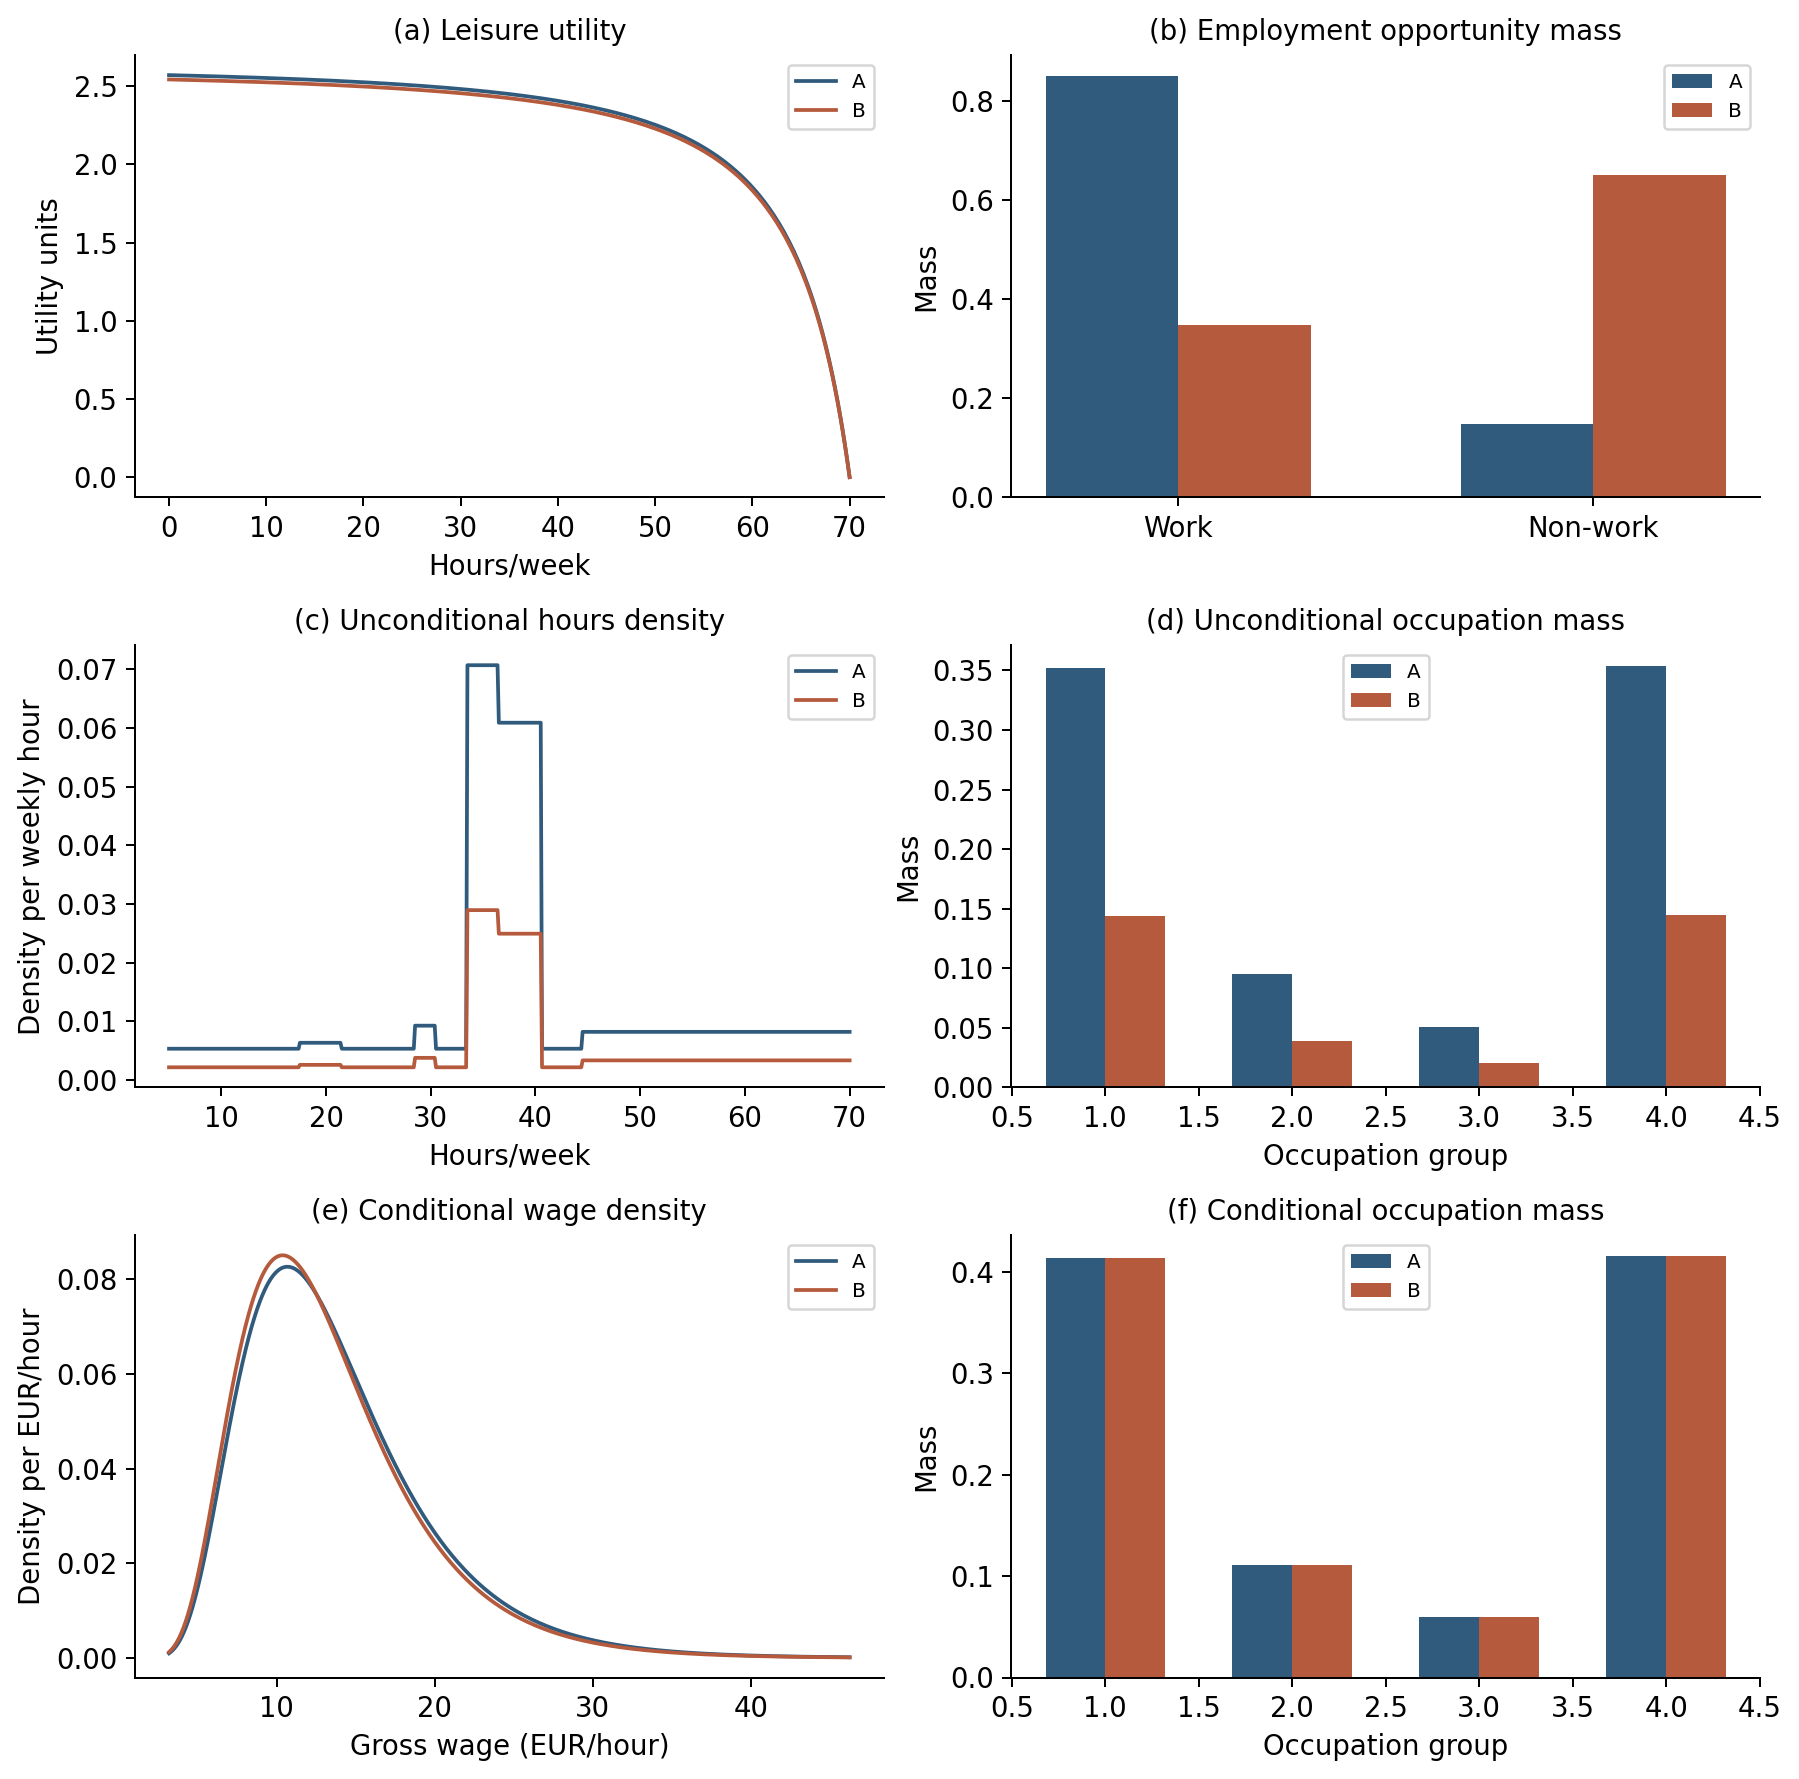
\includegraphics[width=0.95\linewidth,height=\textheight,keepaspectratio,alt={Historical matched employed singles, households A and B (anonymous). The matching restrictions are common employment state, civilian occupation group, model hours band and observed-wage quintile; the forward selection restricts leisure-profile distance to the lowest admissible decile and maximizes opportunity distance. Panels: (a) deterministic leisure utility, utility units; (b) normalized opportunity mass at work and non-work; (c) unconditional working-hours density, per weekly hour, integrating to work mass; (d) unconditional occupation mass, summing to work mass; (e) wage density conditional on work, per EUR/hour, integrating to one; (f) occupation mass conditional on work, summing to one. All opportunities use each household's normalized structural kernel, not its utility-weighted choice distribution. Similar jobs/preferences are not identical. Status: historical model-implied illustration, not corrected or causal evidence.}]{figures/v3/matched_pair.png}
\caption{Historical matched employed singles, households A and B (anonymous). The matching restrictions are common employment state, civilian occupation group, model hours band and observed-wage quintile; the forward selection restricts leisure-profile distance to the lowest admissible decile and maximizes opportunity distance. Panels: (a) deterministic leisure utility, utility units; (b) normalized opportunity mass at work and non-work; (c) unconditional working-hours density, per weekly hour, integrating to work mass; (d) unconditional occupation mass, summing to work mass; (e) wage density conditional on work, per EUR/hour, integrating to one; (f) occupation mass conditional on work, summing to one. All opportunities use each household's normalized structural kernel, not its utility-weighted choice distribution. Similar jobs/preferences are not identical. Status: historical model-implied illustration, not corrected or causal evidence.}
\end{figure}

The six panels distinguish a deterministic leisure-utility curve, opportunity employment mass, unconditional hours density, unconditional occupation mass, conditional wage density and conditional occupation mass. None is a fitted choice probability unless explicitly constructed using \(e^u g/Z\). Multiplying a conditional working density by the opportunity work mass changes its integral; it does not change a density into a point probability. This local interpretation replaces the erroneous four-panel caption.

The illustration belongs before the welfare conclusions because it teaches the distinction used there. It does not identify geography's causal influence, supply a lower bound on all opportunity inequality, or generalize from employed matched singles to couples or actual non-workers. Non-workers also receive an ex-ante evaluation over working and non-working alternatives; observing non-employment does not make their job opportunities irrelevant.

\subsection{Preferences, estimated}\label{preferences-estimated}

The coefficients of the previous section are not themselves the economics. A leisure weight is a coordinate: it changes when the normalizer changes, while the preferences it encodes do not. This section shows the objects that are invariant to that choice, reads each one, and says what it cannot be used for.

\textbf{How to read these panels.} Each is drawn from the estimated utility at a representative household, not from a fitted curve through data. None of them shows a budget set, an opportunity density or a taste shock, so no curve here is a set of attainable bundles and no slope here is a behavioural response. They describe how a household ranks packages; how available those packages are is the next section's question.

\begin{figure}
\centering
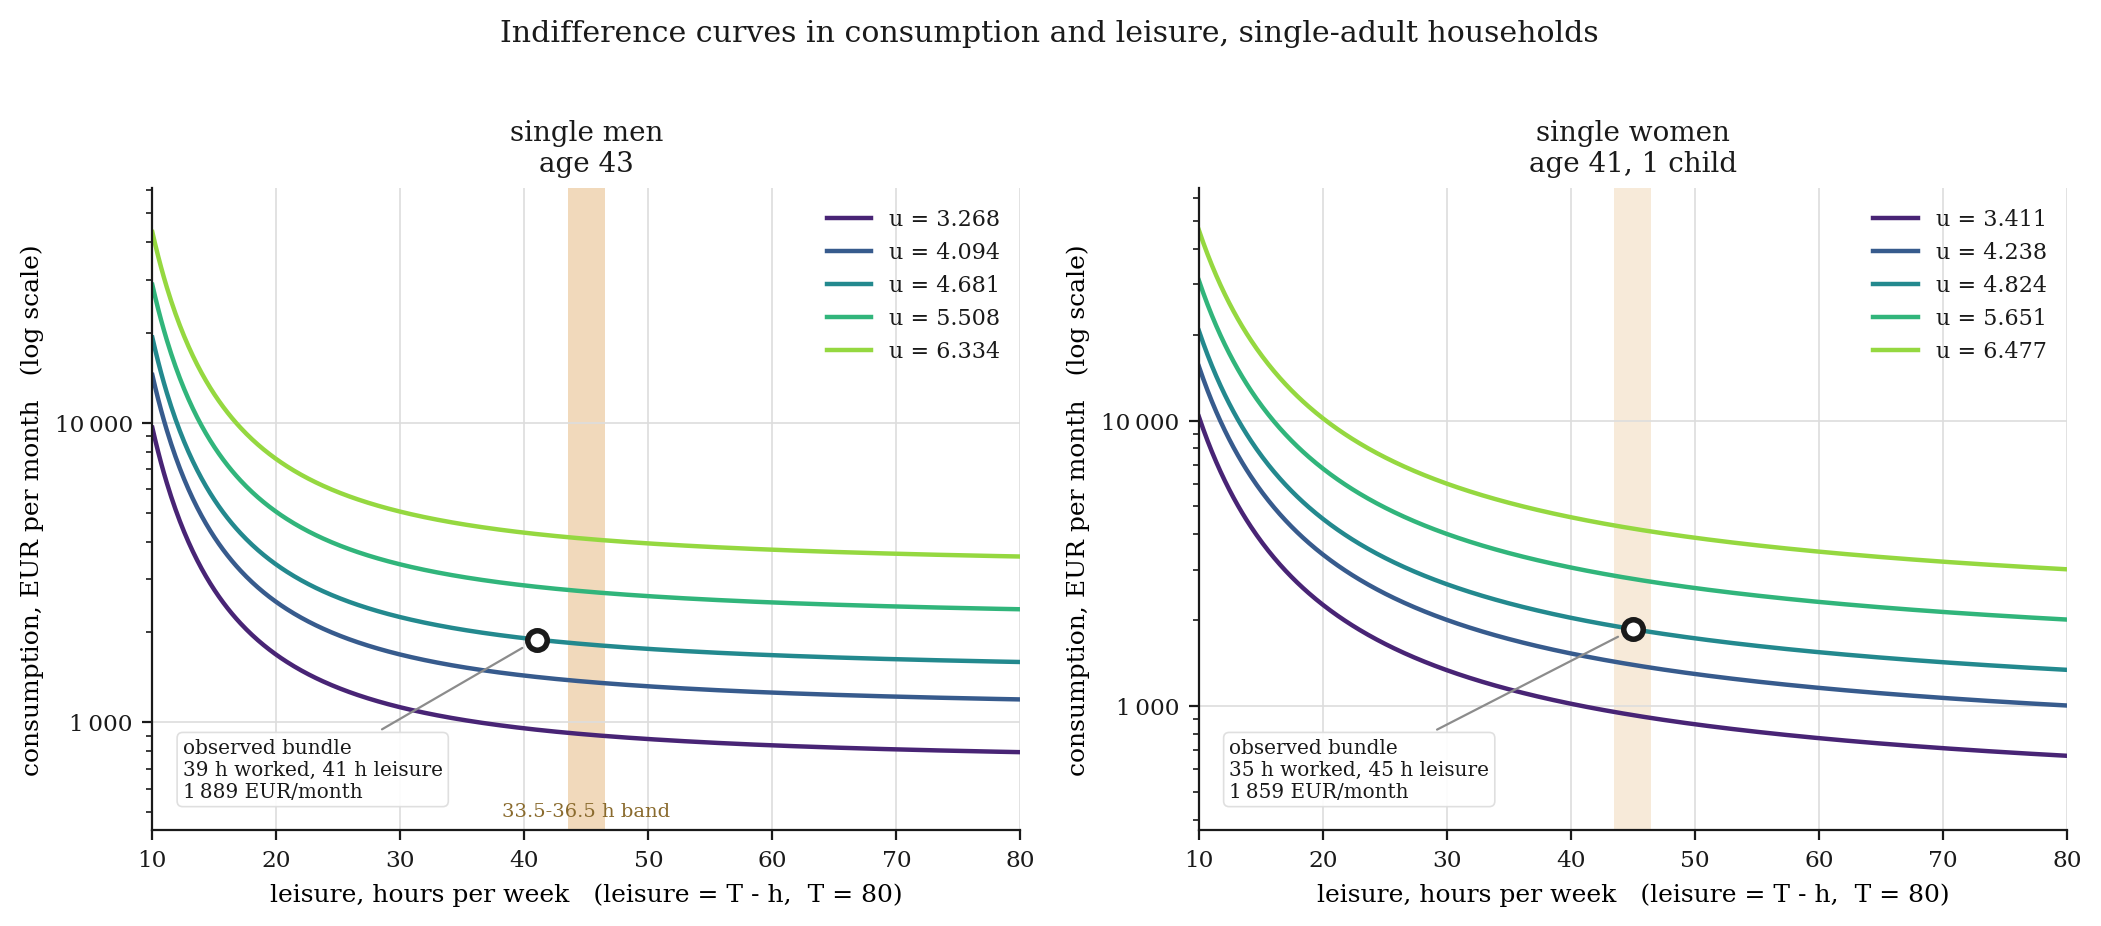
\includegraphics[width=0.95\linewidth,height=\textheight,keepaspectratio,alt={Indifference curves in consumption and leisure, single-adult households. Population: one representative single-adult household of each sex, the medoid of employed deciders on age, hours and consumption. Units: leisure in hours per week, consumption in euros per month. Status: model-implied preference object at the estimated parameters; the budget set, the opportunity density and the taste shock are not drawn, so a curve is not a set of attainable bundles.}]{figures/v3/figP01_indifference_curves_singles.png}
\caption{Indifference curves in consumption and leisure, single-adult households. Population: one representative single-adult household of each sex, the medoid of employed deciders on age, hours and consumption. Units: leisure in hours per week, consumption in euros per month. Status: model-implied preference object at the estimated parameters; the budget set, the opportunity density and the taste shock are not drawn, so a curve is not a set of attainable bundles.}
\end{figure}

Indifference curves for single adults, obtained by exact analytic inversion of the utility rather than as contours of a grid. The observed bundle is marked, so one can see how much consumption would compensate a change in hours at that point. A curve ends where the level set leaves the image of the transform: at very low leisure no consumption attains the level, and the curve is drawn as absent rather than clipped to a value the model does not contain.

\begin{figure}
\centering
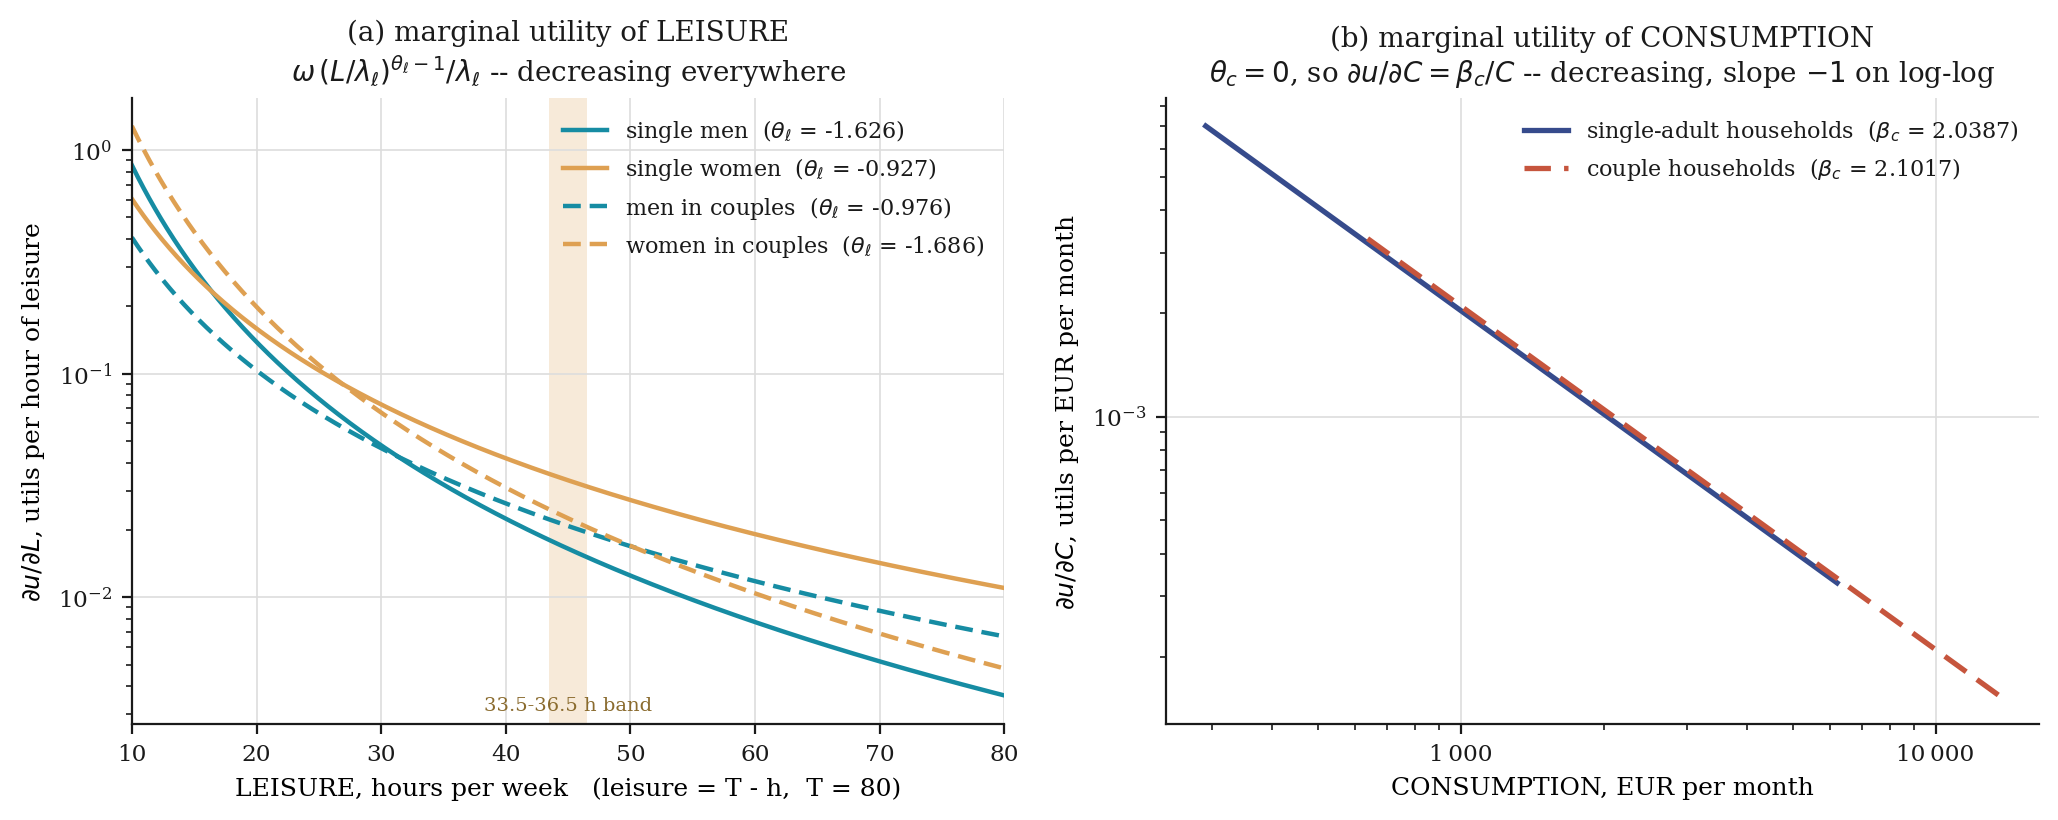
\includegraphics[width=0.95\linewidth,height=\textheight,keepaspectratio,alt={Marginal utility of consumption and of leisure, in physical units. Population: the representative households of each block. Units: marginal utility of consumption per euro per month and of leisure per hour per week, both after the chain-rule conversion from the normalized coordinates. Status: model-implied at the estimated parameters; levels are not comparable across separately estimated utility scales.}]{figures/v3/figP03_marginal_utilities.png}
\caption{Marginal utility of consumption and of leisure, in physical units. Population: the representative households of each block. Units: marginal utility of consumption per euro per month and of leisure per hour per week, both after the chain-rule conversion from the normalized coordinates. Status: model-implied at the estimated parameters; levels are not comparable across separately estimated utility scales.}
\end{figure}

Marginal utilities of consumption and of leisure, converted to physical units by the chain rule. The conversion matters: derivatives with respect to the normalized coordinates are not in euros or hours, and plotting them as if they were is the most common way to misread this model. Levels are not comparable across separately estimated utility scales, so these panels are read within a block and not across blocks.

\begin{figure}
\centering
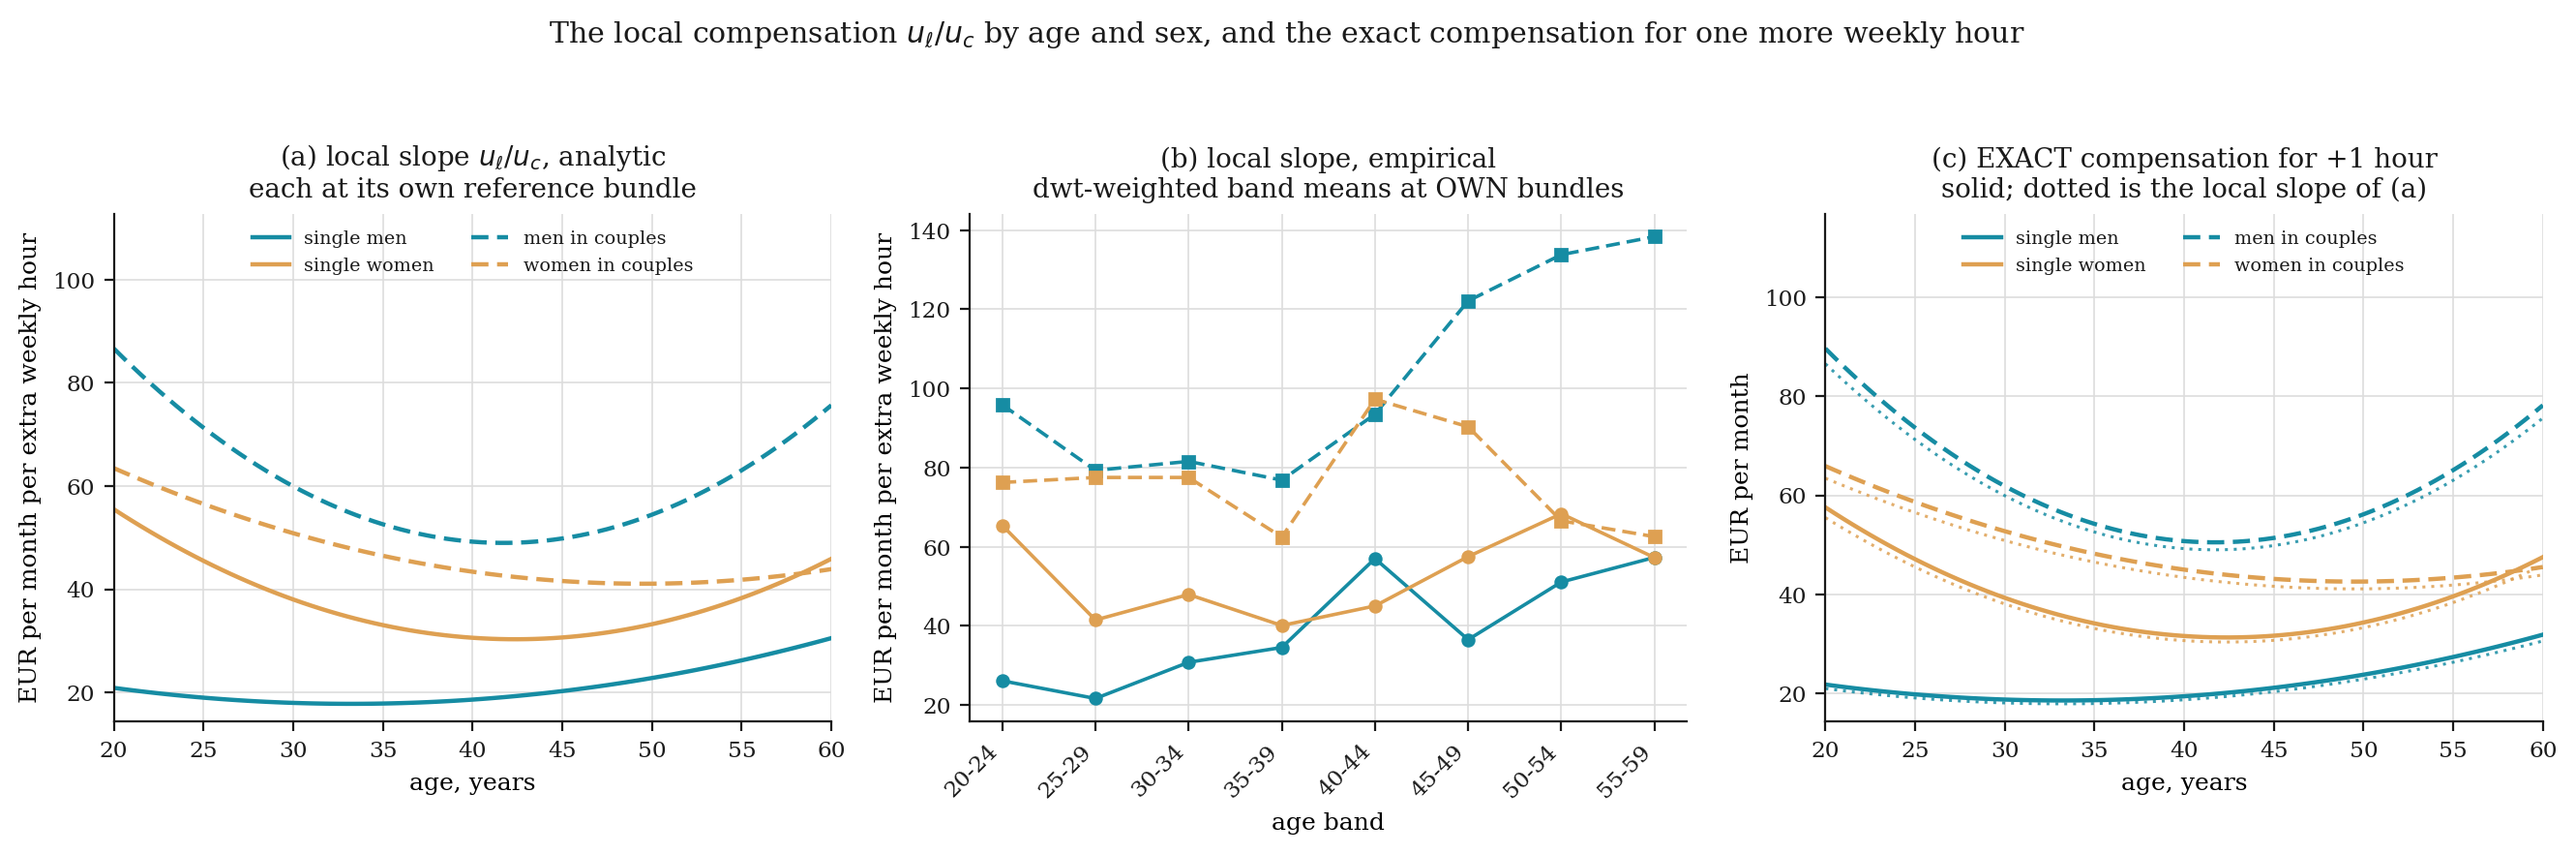
\includegraphics[width=0.95\linewidth,height=\textheight,keepaspectratio,alt={Marginal rate of substitution between leisure and consumption, by age and sex. Population: the representative household profile evaluated across the estimated age range, singles and couples. Units: euros per month of consumption per additional recurring weekly hour of leisure. Status: model-implied at the estimated parameters; a compensation along an indifference curve, not a behavioural response to a wage change.}]{figures/v3/figP04_mrs_by_age_sex.png}
\caption{Marginal rate of substitution between leisure and consumption, by age and sex. Population: the representative household profile evaluated across the estimated age range, singles and couples. Units: euros per month of consumption per additional recurring weekly hour of leisure. Status: model-implied at the estimated parameters; a compensation along an indifference curve, not a behavioural response to a wage change.}
\end{figure}

The compensation for an hour, by age and sex, in euros of monthly consumption per additional weekly hour of work. The panel shows the local compensation, which is the ratio of marginal utilities, alongside the exact compensation for one whole extra hour. The two differ because the first is a derivative and the second is a discrete change, and the gap is the reason the discrete compensations used elsewhere are computed exactly rather than linearised. Note the mixed period: the numerator is monthly and the denominator weekly, so this is not a wage. It is not an elasticity, not a labour-supply response, and not a prediction about how hours would change if a wage changed; those require the budget set and the opportunity density, which are not on this figure.

\begin{figure}
\centering
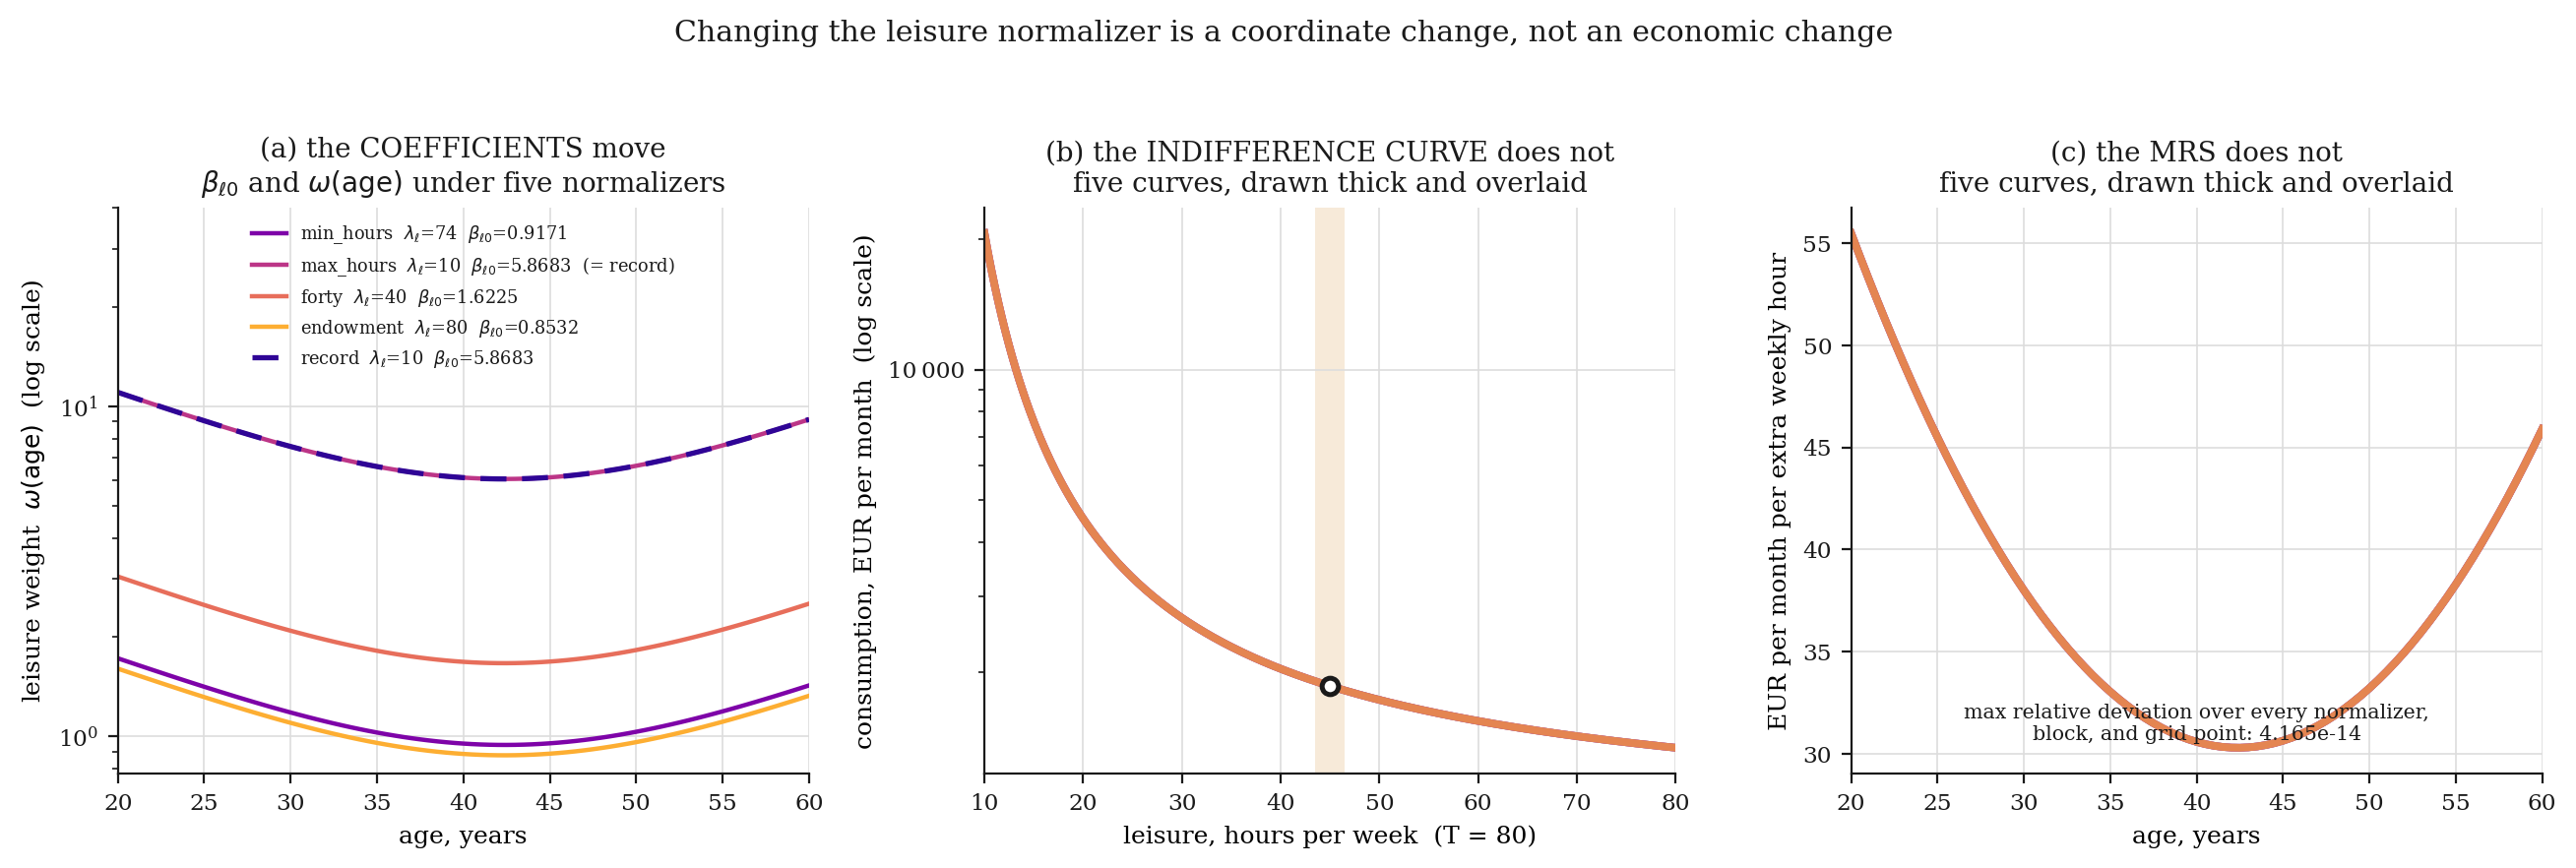
\includegraphics[width=0.95\linewidth,height=\textheight,keepaspectratio,alt={Leisure-normalizer sensitivity: the coefficients move, the indifference curves and the marginal rate of substitution do not. Population: the representative single-adult female household, with the reported deviation maximised over all representative households and every normalizer tested. Units: panel (a) a dimensionless weight on transformed leisure; panel (b) euros per month against hours per week; panel (c) euros per month per extra weekly hour. Status: an exact coordinate change of the estimated model, not a re-estimation; coefficients are coordinates and the curves are the economics.}]{figures/v3/figP06_normalization_sensitivity.png}
\caption{Leisure-normalizer sensitivity: the coefficients move, the indifference curves and the marginal rate of substitution do not. Population: the representative single-adult female household, with the reported deviation maximised over all representative households and every normalizer tested. Units: panel (a) a dimensionless weight on transformed leisure; panel (b) euros per month against hours per week; panel (c) euros per month per extra weekly hour. Status: an exact coordinate change of the estimated model, not a re-estimation; coefficients are coordinates and the curves are the economics.}
\end{figure}

The invariance check, and the reason the previous section's coefficients should not be read as economics. Under a change of leisure normalizer the coefficients move by more than an order of magnitude, while the indifference curves and the marginal rate of substitution coincide. The transformation is exact rather than approximate, and the panel prints the largest deviation found over every normalizer and household tested. One consequence is worth stating precisely, because it is easy to overstate. Re-coordinating multiplies a coefficient and its box endpoint by the same factor, so a coefficient sitting at a bound sits at the transformed bound: the boundary status is unchanged by the normalisation. That is emphatically not the bound being an artefact of the units, and nothing on this panel suggests the constraint is spurious. What settles whether the bound binds is re-estimating with wider bounds, and nothing else.

\section{Money-metric well-being and decomposition}\label{money-metric-well-being-and-decomposition}

\subsection{Welfare: the verified identity and its numerical implementation}\label{welfare-the-verified-identity-and-its-numerical-implementation}

The post-estimation calculation starts from priced consumption and deterministic utility at every integration node. It is ex ante with respect to the distribution of job packages in the specified reference calculation, not the utility of the observed job alone. All integrals use the same mixed job measure. Separate notation is essential:

\[G_{i,S}=\int g_{i,S}d\nu,\quad \widehat g_{i,S}=g_{i,S}/G_{i,S},\quad
Z_{i,S}=\int e^{u_{i,S}}g_{i,S}d\nu,\quad J_{i,S}=Z_{i,S}/G_{i,S},\quad V_{i,S}=\log J_{i,S}.\]

The subscript \(S\) denotes which structural pathways have been equalized. Opportunity mass \(G\), choice normalizer \(Z\), normalized utility integral \(J\) and its logarithm \(V\) are not interchangeable. In particular, \(\log Z\) responds to a common multiplication of every opportunity intensity, whereas \(\log J\) does not. An expected-maximum interpretation would require the additional stochastic foundation noted above; the implemented functional itself is fully defined by these integrals.

\subsubsection{The monetary reference and its closed form}\label{the-monetary-reference-and-its-closed-form}

Write deterministic utility as \(u_{i,S}(j)=L_{i,S}(j)+BC(C_{i,S}(j)/\lambda_c;\theta_c)\), where \(L\) contains the entire non-consumption component, including both spouse leisure terms for couples. The reference gives \textbf{one flat monthly disposable-consumption amount to every alternative} while retaining that state's \(L\) and \(\widehat g\). Define

\[H_{i,S}=\int e^{L_{i,S}(j)}\widehat g_{i,S}(j)d\nu(j),\qquad
\Phi_{i,S}(m)=BC(m/\lambda_c;\theta_c)+\log H_{i,S}.\]

Money-metric equivalent income \(W_{i,S}\) is the positive monthly euro amount satisfying \(\Phi_{i,S}(W_{i,S})=V_{i,S}\). It is not an hourly wage offer, gross earnings transfer, budget-line intercept before tax, or consumption at a fixed leisure point. The factorization follows because the reference consumption term is constant across alternatives and can be taken outside the integral. With the maintained consumption coefficient equal to one,

\[\boxed{W_{i,S}=\lambda_c\left[1+\theta_c\{\log J_{i,S}-\log H_{i,S}\}\right]^{1/\theta_c}},\qquad\theta_c\ne0.\]

This identity has now been checked against the executed evaluator for both household types in every principal preference/environment state: maximum absolute difference \(3.7\times10^{-10}\) euros per month over 15,320 household-states. The test uses historical parameter vectors and already-priced common support, so it verifies the identity and its implementation, not corrected economic estimates. The small discrepancy is numerical stopping and floating-point error. The solver rerun also reproduces the stored evaluated values.

For the couple model's logarithmic consumption utility, the limiting expression simplifies further:

\[\boxed{W_{i,S}=\lambda_c e^{\log J_{i,S}-\log H_{i,S}}
=\frac{\int C_{i,S}(j)e^{L_{i,S}(j)}\widehat g_{i,S}(j)d\nu(j)}
{\int e^{L_{i,S}(j)}\widehat g_{i,S}(j)d\nu(j)}}.\]

Thus the log-consumption special case is an arithmetic consumption average weighted by \(e^L\widehat g\), normalized to integrate to one. It is not a geometric mean, a mean under choice probabilities, or a consumption average that ignores leisure. The single-adult Box--Cox expression is its nonlinear counterpart. The numerical inversion in the production implementation solves this same identity; it is not a second welfare object.

\subsubsection{The stochastic extension, and what it replaces}\label{the-stochastic-extension-and-what-it-replaces}

The normative principle defines the reference by a \emph{maximum} over the individual's set at a flat consumption level. The object evaluated above is an \emph{integral}. These are different functionals. What is evaluated here is therefore not an implementation of the theoretical measure but its \textbf{stochastic, ex-ante extension}, and we do not claim that the theoretical characterisation transfers to it. To keep the two apart we write \(W^1\) for the theoretical measure and \(W^{1\text{-EA}}\) for the extension, never the bare symbol for both, and never call the empirical object literally \(W^1\).

Three clauses of the principle are preserved: the household's own opportunity environment is retained, its own preferences select on both sides of the inversion, and pay is neutralised in the reference \emph{index}. Three things change, and one is added. The set becomes a support \textbf{and} a density, so the weights do work a 0/1 set cannot. The maximum becomes a log-sum-exp. The realised bundle becomes an ex-ante value that excludes the observed chosen row. And idiosyncratic shocks, absent from the theory statement, are added.

\textbf{The attainment that is evaluated.} \(V_i\) is the ex-ante value over the household's own opportunity distribution, and the basis excludes the deterministic chosen row. \(W^{1\text{-EA}}\) therefore answers \emph{what flat pay, offered at every job the household could draw, makes its prospect as good as the prospect it faces}. It does not answer a question about the job the household actually holds.

\textbf{A flat level makes two measures closed-form.} Because the reference level is constant across alternatives, the consumption term leaves the log-sum. Writing \(\Lambda_i=\log H_i\) and \(L_i(\text{home})\) for the taste index at non-work, and letting \(W^{4\text{-EA}}\) denote the staying-home equivalent on the same ex-ante basis --- a reference that neutralises only the \emph{direct} dependence of the reference on the opportunity set, never its effect through the attained outcome ---

\[BC(W^{1\text{-EA}}_i/\lambda_c)=V_i-\Lambda_i,\qquad BC(W^{4\text{-EA}}_i/\lambda_c)=V_i-L_i(\text{home}),\]

so the entire difference between them is one scalar per household, \(\Delta_i=L_i(\text{home})-\Lambda_i\). Derived this way the two expressions reproduce the certified evaluator's \(W^4\) exactly and its \(W^1\) to a relative \(4\times10^{-14}\), so this reads the implemented object rather than re-implementing it.

\textbf{A coincidence in the small-shock limit, and why it does not bind here.} On the estimated preference domain --- leisure positively valued, no intrinsic value of work beyond the leisure term, non-work always available --- non-work is the deterministic maximiser of the reference taste index. This was checked rather than assumed and holds for every household in the sample on which the check could be run. Consequently \(\lim_{\tau\to0}W^{1\text{-EA}}=W^{4\text{-EA}}\) exactly. This is a \textbf{mathematical limit of the stochastic construction}: it says what the measure would become if the idiosyncratic shocks were shrunk to nothing. It is not an estimate, not a scenario, and not something done to the data anywhere in this paper. Throughout, \(\tau\) is the scale of the idiosyncratic shocks; \(\sigma\) is reserved for the dispersion of the wage-offer distribution and is a different object.

The two are nevertheless distinct at the estimated scale, because \(W^{1\text{-EA}}\) integrates where \(W^{4\text{-EA}}\) maximises, and the separation is carried entirely by that smoothing. We do not put a number on it here. The statistics that compared the two measures in earlier drafts were computed under a different scale convention, a different support and a different sample, and they have been returned for reconciliation against the corrected frame; no ratio between the two measures is printed in this document until that returns. One specific claim is withdrawn rather than merely deferred: the earlier statement that the household gap \(\Delta_i\) is negative for every household does not hold on the corrected frame for single adults, where the sign is not uniform, though it does hold throughout the couples panel. We report the coincidence as a property of the measure under freely available non-employment, not as a defect repaired by adding accessibility thresholds or job amenities.

\textbf{The utility scale is identified, and this closes the question the bridge raised.} An earlier version of this argument had to record the shock scale as a normalisation: with the consumption weight fixed at one as a numeraire, \(\tau\) was not separately identified, and the separation of \(W^{1\text{-EA}}\) from \(W^{4\text{-EA}}\) rested on a scale nobody had estimated. That is no longer the position. Fixing \(\tau=1\) and the consumption curvature at zero, and estimating the consumption weight instead, identifies the scale: \(\beta_c\) is 2.03873 (standard error 0.291729) for single-adult households and 2.10172 (0.293879) for couples. The restriction is not free-standing algebra: it improves the likelihood by 23.7526 and 15.659 log-points, and the population fit improves with it, from 0.01523 to 0.01304 for singles and from 0.01385 to 0.013595 for couples.

Under log consumption a unit of the shock scale is \emph{proportional}, not additive: one nat maps to \(C'=C\exp(1/\beta_c)\), a rise of 63.3 per cent in consumption for singles and 60.9 per cent for couples, at whatever level it is applied. That proportional form is the scale-free statement and is how the nat should be read. In ratio form the factor is 1.633 for singles and 1.609 for couples. A euro amount exists only against a stated baseline: evaluated at the corrected chosen-consumption median of EUR 1,760.63 per month, one nat carries a single-adult household to EUR 2,875.34; for couples, from EUR 3,854.22 to EUR 6,202.61. Quoted without its baseline, either euro figure means nothing. The money metric is therefore reported on an estimated scale. No declared-scale sensitivity is required, because the scale is no longer declared.

\textbf{What the estimated order does to the measure.} At \(\theta_c=0\) the measure is a power mean of order \(\beta_c\) of the consumption attached to the alternatives a household can reach. The order is doing two jobs at once, and this is what makes the estimate economically substantive rather than a fitting constant: \(\beta_c\) is simultaneously the order of the mean and the elasticity of an alternative's implied weight with respect to its own consumption. At the estimate an alternative paying twice the median carries 4.11 times the weight of the median alternative, not twice it; across the observed fifth-to-ninety-fifth percentile span of reachable consumption the implied weight ratio is 95.6 to one, against 9.4 to one under an arithmetic mean. By the power-mean inequality an order above one raises the measure relative to the arithmetic mean and tilts it toward the best-paying alternatives a household can actually reach. Two limits belong with this reading and should travel with the panel that draws it. The power-mean representation exists only at \(\theta_c=0\); away from that restriction the aggregator has no such closed form. And the panel varies \(\beta_c\) inside the aggregator's kernel, holding the estimated model fixed --- it shows what the weighting would do at other orders, and is not a re-estimation of the model under \(\beta_c=1\).

\textbf{What the reference does and does not neutralise.} The reference neutralises pay \emph{in the utility index}: the Box--Cox consumption term is constant across alternatives, so job pay enters the reference utility nowhere. It does not follow that the measure as a whole is pay-free. The wage is a coordinate of the alternative, so it survives in the opportunity density after being neutralised in utility, and equalising the wage block moves \(W^{1\text{-EA}}\) by up to EUR 438, or 34 per cent, for some households. Because the reference index is pay-free by construction, that movement can only travel through the opportunity distribution. Separating the direct reference-set channel from the indirect attainment channel within that movement requires knowing whether the household's own attainment normalizer \(H_i\) is invariant to the equalisation, and it is. Because the bounded wage density is normalized and the non-consumption utility carries no wage term, the largest household \(|\Delta\log H_i|\) found is 1.8e-15 for singles and 7.1e-15 for couples --- numerical zero in both, though not the same numerical zero, and we quote each rather than the smaller of the two. The direct channel accordingly moves the median household by EUR 0 exactly, and the entire movement travels through attainment: a median of EUR -17.43 for singles and EUR +110.53 for couples. The licensed statement is therefore that \emph{the reference is directly pay-neutral, while earning opportunities affect the measure through attainment} --- which is the same distinction drawn axiomatically in the introduction, now measured. The accurate statement, used throughout, is therefore: \emph{the reference neutralises pay differences in the utility index, while a residual pay channel reaches the measure through the wage limb of the opportunity distribution.} Two consequences bind how the results are read. Earning opportunities are a component of the stochastic opportunity distribution, not a separate pay schedule outside it. And \(W^{1\text{-EA}}\) accordingly \textbf{does not inherit independence of pay} from the theoretical measure: that property holds of the reference index, and the stochastic extension does not carry it.

\textbf{Frame.} These magnitudes come from a certified evaluation that is not the final corrected frame. The closed forms and the small-shock limit are algebraic and hold on any frame; the magnitudes are specific to the one they were computed on.

\subsubsection{Existence, precision and what opportunity changes can do}\label{existence-precision-and-what-opportunity-changes-can-do}

The derivative \(\Phi'(m)=(m/\lambda_c)^{\theta_c-1}/\lambda_c\) is positive for positive \(m\). Hence a root is unique on its permitted domain. The Box--Cox inverse base must be positive, and the attained value must fall within the reference range. On a finite positive-consumption panel the reference values at the smallest and largest priced consumption bracket the attained value; this gives the economic reason for a bracket check. The identity audit found a strictly positive inverse base throughout its singles calculations. A finite realised panel alone does not prove the existence of the population integral on unbounded wages.

Numerical integration averages importance-corrected contributions over the common nodes, then takes the logarithm and inverse; it does not average the inverse of each node or each scramble. The same opportunity/proposal correction enters \(J\) and \(H\). Any common mass normalization or common node-count factor cancels from their ratio. The integration support excludes the staged chosen row, whose contribution is exactly zero. The chosen-row estimation defect therefore does not contaminate this integrator mechanically, although a changed estimate changes its downstream economic answer.

There is no unconditional theorem that a wider opportunity set raises this metric. Opportunities affect attained value and the reference map simultaneously. In the logarithmic case, adding weight on consumption below the existing weighted average can lower \(W\). If all alternatives have the same consumption \(C_0\), the identity gives \(W=C_0\) regardless of the opportunity intensities. Commonly multiplying \(g\) also leaves \(W\) unchanged. These are algebraic consequences of the implemented definition, not empirical assertions about a reform. Improving actual disposable consumption pointwise with the reference otherwise fixed raises the measure; that different statement follows from its monotonicity.

\subsubsection{A calculation from the current evaluator, in parallel}\label{a-calculation-from-the-current-evaluator-in-parallel}

The following examples select an anonymous median-value household within each type from the historical evaluator. No household identifiers or detailed demographic profile are exported. Displayed jobs are simulated integration nodes, already priced under the historical budget; they are not the observed jobs or an exhaustive job menu. The single example is a female single-adult household; the couple example includes all joint regimes. Historical singles consumption still has the aggregation limitation described in the data section. This is a worked current-evaluator calculation, not corrected empirical evidence.

Worked historical-evaluator examples. Population: one anonymous median-value single woman and one couple; jobs: selected simulated nodes; hours/week (man/woman for couples), priced consumption EUR/month, non-consumption utility L in utility units; remaining columns: normalized numerical node masses on each household's own common support. Reference: own flat consumption; status: model-implied at historical parameters, not corrected findings.

{ % do not increment counter
\small\setlength{\tabcolsep}{3pt}\begin{longtable}[]{@{}>{\raggedright\arraybackslash}p{0.1000\linewidth}>{\raggedright\arraybackslash}p{0.1350\linewidth}>{\raggedright\arraybackslash}p{0.1350\linewidth}>{\raggedright\arraybackslash}p{0.1350\linewidth}>{\raggedright\arraybackslash}p{0.1350\linewidth}>{\raggedright\arraybackslash}p{0.1350\linewidth}>{\raggedright\arraybackslash}p{0.1350\linewidth}@{}}
\toprule\noalign{}
Type & Hours & Consumption & L & Opportunity & Choice & Reference \\
\midrule\noalign{}
\endhead
\bottomrule\noalign{}
\endlastfoot
Single & 0.0 & 526.02 & 3.9001 & 0.00023 & 0.00016 & 0.00037 \\
Single & 35.0 & 961.62 & 3.5019 & 0.00104 & 0.00083 & 0.00114 \\
Single & 70.0 & 2676.77 & 0.0104 & 0.00055 & 0.00004 & 0.00002 \\
Single & 20.0 & 992.44 & 3.7318 & 0.00012 & 0.00012 & 0.00017 \\
Couple & 0.0/0.0 & 543.51 & 7.0302 & 0.00004 & 0.00002 & 0.00007 \\
Couple & 39.1/0.0 & 311.24 & 6.6780 & 0.00035 & 0.00009 & 0.00050 \\
Couple & 0.0/19.3 & 1269.72 & 6.9684 & 0.00016 & 0.00022 & 0.00030 \\
Couple & 38.7/35.4 & 2498.61 & 6.5027 & 0.00028 & 0.00048 & 0.00034 \\
\end{longtable}
}

The opportunity column is each node's normalized importance-corrected contribution to \(G\); the choice column normalizes \(e^u\) times that contribution. The reference column normalizes \(e^L\) times it. They are numerical node masses, not continuous density heights or the probability of receiving that exact wage--hours pair. The displayed subset does not sum to one because the full integration contains the remaining nodes. Repeated representations of the non-work atom must be aggregated before interpreting its total mass.

Same anonymous households through the principal equalization states. Population: the examples immediately above; measure: normalized log integrals (dimensionless) and equivalent income (EUR/month); reference: each state's flat-consumption map; status: model-implied historical-parameter evaluator outputs, not population inequalities.

{ % do not increment counter
\small\setlength{\tabcolsep}{3pt}\begin{longtable}[]{@{}>{\raggedright\arraybackslash}p{0.2500\linewidth}>{\raggedright\arraybackslash}p{0.1650\linewidth}>{\raggedright\arraybackslash}p{0.1650\linewidth}>{\raggedright\arraybackslash}p{0.1650\linewidth}>{\raggedright\arraybackslash}p{0.1650\linewidth}@{}}
\toprule\noalign{}
Type & State & log J & log H & W (EUR/month) \\
\midrule\noalign{}
\endhead
\bottomrule\noalign{}
\endlastfoot
Single & baseline & 3.14536 & 3.40517 & 1360.54 \\
Single & preferences & 3.87947 & 4.16789 & 1320.34 \\
Single & environment & 3.14667 & 3.46102 & 1284.76 \\
Single & all & 3.89573 & 4.23506 & 1251.25 \\
Couple & baseline & 5.53703 & 6.30227 & 1777.82 \\
Couple & preferences & 5.36884 & 6.13396 & 1778.04 \\
Couple & environment & 5.49386 & 6.30248 & 1702.34 \\
Couple & all & 5.33144 & 6.13373 & 1713.16 \\
\end{longtable}
}

For example, the displayed baseline entries give the following explicit substitutions (rounding is for exposition only):

\[\begin{aligned} W_{\rm single}&\simeq 1774.52\left[1+0.168019(3.14536-3.40517)\right]^{1/0.168019}\simeq 1360.54\ \text{EUR/month},\\W_{\rm couple}&\simeq 3821.45\exp(5.53703-6.30227)\simeq 1777.82\ \text{EUR/month}.\end{aligned}\]

Starting with the baseline row, subtract \(\log H\) from \(\log J\) and apply the boxed inverse using the registered consumption scale and curvature. In the single example the scale is 1774.52 euros/month and the curvature 0.168019; the couple example uses the logarithmic case and scale 3821.45 euros/month. For couples the same result is obtained by summing priced consumption times the reference column over all nodes. Preference equalization changes \(L\) on both sides; environment equalization changes opportunities and priced budgets using the declared reference operands; the full state changes both. The table uses the same household through these states. Its numbers are a reproducible diagnostic at existing estimates, not the missing corrected distributional attribution.

One source difference remains consequential: the existing singles welfare panel's consumption scale differs from the estimation-frame scale. The evaluator reads the panel's actual scale, which correctly converts its stored normalized consumption back into euros; the worked calculation reports that value. The identity check does not establish that using the unchanged parameter vector on differently scaled consumption preserves the estimated behavioural model. That estimation-to-welfare scale equivalence must be reconciled in the corrected rebuild, rather than assumed from a comment calling the scale numerical. This does not invalidate the verified algebra of the current evaluator, but limits its interpretation as welfare from the corrected estimated model.

\subsection{Interpersonal comparison, household welfare and equivalization}\label{interpersonal-comparison-household-welfare-and-equivalization}

The baseline monetary comparison retains each household's preferences and opportunity distribution in its own flat-consumption reference. It gives a common operational meaning to the monetary amount: disposable consumption at every reference alternative. A difference in euros is a difference in that specified amount. It is not automatically an equal difference in subjective utility, a transferable compensation payment or an interpersonal comparison justified solely by the currency unit.

Actual earning opportunities still affect priced consumption and attained value even though the reference replaces actual alternative-specific consumption. Reference flattening does not erase the actual budget's earnings effects. Equally, a reference preserving own opportunities need not rank menu changes like a fixed common-opportunity reference. The baseline and a common-preference counterfactual therefore answer different questions; neither is silently substituted for the other.

The welfare unit for couples is the household. The unitary model supplies no empirical allocation of this welfare between partners and no within-couple inequality measure. Comparison of a couple's household amount with a single adult's amount needs an explicit needs adjustment. The implemented modified-OECD scale is

\[e_i=1+0.5(N_{i,\ge14}-1)+0.3N_{i,<14},\qquad W_i^{\rm eq}=W_i/e_i,\]

where \(N_{i,\ge14}\) and \(N_{i,<14}\) count household members by the scale's cutoff. This cutoff is distinct from the child regressor's definition. The welfare weights remain household survey weights; an individual-weighted analysis would be another population.

When composition is equalized, the needs scale follows the same counterfactual roster. This keeps the budget-side household and the needs denominator economically aligned. Zero residual inequality in a grand coalition, where obtained, is a consequence to check, not a normative justification for the choice. Holding the scale at its own value or treating scale as a separate factor would define different games and can be mathematically coherent if every pathway is assigned explicitly. It is incorrect to claim those alternatives necessarily double-count or cannot close.

Raw and equivalized within-type inequality are both useful. Pooled singles--couples inequality additionally requires a cross-type reference that makes the household interpretations comparable. A failure of one previously tested pooled reference does not prove all pooling impossible, but neither may type-specific offsets be added simply to force an exhaustive identity. Corrected pooled results and their reference basis remain pending.

\subsection{Weighted inequality and the choice of index}\label{weighted-inequality-and-the-choice-of-index}

For positive household equivalent incomes, the implemented weighted Gini is

\[I(W)=\frac{\sum_i\sum_j\omega_i\omega_j|W_i-W_j|}{2\sum_i\omega_iW_i},\qquad\sum_i\omega_i=1.\]

The weights are the household survey weights defined before the descriptive statistics. The numerator averages absolute pairwise differences and the denominator scales them by twice mean well-being. The index is dimensionless; a contribution expressed in Gini points is not a percentage until divided by the stated baseline index. No unreported finite-sample correction is appended to this normalized-weight formula. Non-positive values or a non-positive denominator require explicit domain handling, not silent exclusion.

The index treats proportional rescaling of all positive equivalent incomes as leaving inequality unchanged. An income Gini and a well-being Gini still concern different distributions: the former does not value leisure or integrate opportunities under the declared reference. Their difference is not itself a causal opportunity effect. The Gini is used for a transparent common distributional scale; an Atkinson index would add explicit inequality-aversion choices, and generalized-entropy measures would change tail sensitivity and decomposability. Those alternatives change the economic weighting of differences. No uncomputed alternative-index numbers are supplied.

Integration uncertainty is assessed by re-evaluating this final statistic after leaving out a scramble, rather than averaging household numerical errors. Parameter uncertainty requires recalculating household welfare and inequality under parameter draws. Reference sensitivity instead compares complete calculations using alternative normative profiles. Keeping these operations separate matters especially when the denominator of a reported share also changes.

\subsection{Equalization operators and their pathways}\label{equalization-operators-and-their-pathways}

Counterfactual equalization replaces specified structural inputs by declared reference operands without re-estimation. It is not a wholesale replacement of a household's raw record every time one covariate appears in a channel. Singles additionally select the complete estimated reference-sex preference block when preferences are equalized; couples retain each spouse's coefficient block and substitute its reference arguments. The broad environment comprises access \(A\), wage opportunities \(B\) and budget endowments/needs \(D\); the preference block is \(P\). The budget block's resources/needs subdivision is resolved for single-adult households on the corrected pathway assignments and repricing, and remains unavailable for couples.

Structural equalization operators for both household types. Measure: input substitutions, not causal effects; units inherited from each input; reference: selected representative profile and coalition-consistent monetary map; status: extracted broad operators. The resources/needs subdivision is resolved for single-adult households and unavailable for couples.

{ % do not increment counter
\small\setlength{\tabcolsep}{3pt}\begin{longtable}[]{@{}
  >{\raggedright\arraybackslash}p{(\linewidth - 8\tabcolsep) * \real{0.2000}}
  >{\raggedright\arraybackslash}p{(\linewidth - 8\tabcolsep) * \real{0.2000}}
  >{\raggedright\arraybackslash}p{(\linewidth - 8\tabcolsep) * \real{0.2000}}
  >{\raggedright\arraybackslash}p{(\linewidth - 8\tabcolsep) * \real{0.2000}}
  >{\raggedright\arraybackslash}p{(\linewidth - 8\tabcolsep) * \real{0.2000}}@{}}
\toprule\noalign{}
\begin{minipage}[b]{\linewidth}\raggedright
Operator
\end{minipage} & \begin{minipage}[b]{\linewidth}\raggedright
Replaced / profile
\end{minipage} & \begin{minipage}[b]{\linewidth}\raggedright
Household-specific remainder
\end{minipage} & \begin{minipage}[b]{\linewidth}\raggedright
Repricing
\end{minipage} & \begin{minipage}[b]{\linewidth}\raggedright
Reference map
\end{minipage} \\
\midrule\noalign{}
\endhead
\bottomrule\noalign{}
\endlastfoot
Preferences P & Singles: weighted mean index arguments and complete reference-sex coefficient/curvature block. Couples: medoid spouse arguments, own spouse coefficients & Budget roster, resources, access and wage shifters unless separately equalized & No for pure utility shifters & Replace L on both sides \\
Access A & Singles: weighted mean access arguments and marginalized normalized occupation table. Couples: medoid market arguments & Preferences, wage locations, budget inputs; couple sex-specific occupation coefficients remain & No for pure access indices & Replace opportunity weights on both sides \\
Wage opportunities B & Singles: weighted education shares and experience moments. Couples: medoid spouse education/experience; squares recomputed. Estimated wage coefficients retained & Preference and access pathways of same covariates & Not from an index change alone on common priced jobs & Replace wage weights on both sides \\
Budget D & Policy inputs from representative budget household, including resource and needs pathways & Non-D structural pathways & Yes; rerun household budget & Use new consumption in J; state L and opportunities in H \\
Resources within D & Corrected resource fields and take-up; work-history priority pending & Composition/needs unless separately changed & Yes when policy inputs change & No independent new reference; follow resulting state \\
Needs within D & Roster/needs and linked scale, selected needs profile & Resource and utility-child pathways unless separately changed & Yes; update needs scale & Follow resulting state; no hidden P change \\
\end{longtable}
}

The reference construction genuinely differs across the two applications. Singles use survey-weighted means of the access, wage and preference index arguments. The mean squared-age or squared-experience argument is retained as a separate moment, not replaced by the square of the mean. The occupation-access substitution uses the normalized occupation table marginalized over its equalized conditioning coordinates. Singles' primary preference reference selects the full female coefficient/curvature block after the shifters are equalized; its child term then applies commonly, including to men. The male structural-zero arm is a sensitivity exercise, not a value to average with it. This is a common index profile, not an actual synthetic household guaranteed feasible for tax pricing.

For budget pricing, the reference instead is an actual representative household, selected as a survey-weighted medoid. Continuous household-input differences are divided by their weighted interquartile range; categorical inputs contribute mismatch indicators. The selected household minimizes the weighted total distance, with a deterministic profile-based tie-break. Singles use household sums and decider categories; couples use household sums and both spouses' categories where necessary. Couple structural substitutions use that medoid's corresponding spouse arguments, never cross-sex coefficient averages. These differences must remain visible when comparing their attribution, even though the welfare identity is shared.

The pathway rule is essential. Age can enter leisure preferences, experience-dependent wage locations and policy eligibility. Education can enter the wage equation and the group-unemployment lookup. Children can enter female leisure utility, the household budget and the needs scale. Equalizing the preference pathway of children changes the utility shifter, not the tax roster. Equalizing earnings opportunities changes their structural wage shifters, not preferences or the employment-access lookup. Equalizing composition changes the budget/needs pathway, not a preference shifter unless \(P\) is also in the coalition. Pure preference-shifter substitution therefore does not automatically require repricing.

Conversely, moving a policy input that changes entitlement requires new budget evaluation. Work-history fields overwritten by the alternative's employment state cannot also be independently equalized as fixed resources without a declared priority and economic interpretation. Correcting the fringe-benefit, company-car and imputed-rent classifications is necessary but does not alone resolve that operator dependency. The prior nested resource/needs percentages are withdrawn, not relabelled as current. For single-adult households the dependency is now resolved on the corrected partition and the repriced panels, so a corrected resources share and a corrected composition-and-needs share are established and reported below. For couples no separately repriced partial pair exists, so neither couples share is established and the cells are marked rather than imputed.

In every coalition, the same state's non-consumption utility and opportunities enter both attained value and its flat-consumption reference map. The reference map is recalculated when those inputs change. \(q\), numerical centring constants and integration normalizers are not independent economic factors to equalize. A different assignment of pathways is a different decomposition, not a silent robustness adjustment.

\subsection{Grouped attribution and interactions}\label{grouped-attribution-and-interactions}

Start with the preference block \(P\) and the broad non-preference block \(E=\{A,B,D\}\). Let \(I_{00}\) be baseline inequality, \(I_{10}\) inequality after preferences are equalized, \(I_{01}\) after the environment is equalized, and \(I_{11}\) after both. Equalizing a factor does not necessarily reduce inequality. The one-factor preference change is \(I_{00}-I_{10}\); the environment change is \(I_{00}-I_{01}\). The two-player Shapley allocations are instead

\[C_P=\tfrac12[(I_{00}-I_{10})+(I_{01}-I_{11})],\qquad
C_E=\tfrac12[(I_{00}-I_{01})+(I_{10}-I_{11})].\]

Each averages the factor's marginal effect when moved first and when moved second. Thus \(C_P+C_E=I_{00}-I_{11}\), and shares divided by \(I_{00}\) sum to \((I_{00}-I_{11})/I_{00}\), not necessarily one. Signed allocations are allowed. Calling \(C_E/I_{00}\) the percentage removed by equalizing the environment would confuse attribution with the one-factor counterfactual.

Within the environment group, the grouped allocation averages over orders of access, wage opportunities and budget endowments/needs while keeping the environment group contiguous relative to preferences. If \(v(S)=I(\varnothing)-I(S)\) and \(\Pi_{\mathcal G}\) is the set of orderings that respect the declared grouping, the operational averaging is

\[C_k=\frac{1}{|\Pi_{\mathcal G}|}\sum_{\pi\in\Pi_{\mathcal G}}
\left[v(\operatorname{Pred}_\pi(k)\cup\{k\})-v(\operatorname{Pred}_\pi(k))\right].\]

\(\operatorname{Pred}_\pi(k)\) denotes the factors preceding \(k\) in ordering \(\pi\). The grouping makes the preference--circumstance distinction primary and prevents an arbitrary proliferation of circumstance labels from changing that top-level comparison. It is an explicit ethical/accounting design, not something learned from the likelihood. A flat Shapley game would allocate some interactions differently. A further resources/needs split must preserve the declared hierarchy and use correctly repriced coalitions, not rescale pieces to recover old totals.

The narrower market-opportunity allocation is \(C_A+C_B\). Resources and needs remain separate non-preference contributions. Geography can be nested within access under a declared operator, but a geographic component is neither a causal instrument nor a lower bound on all opportunity inequality. Algebraic exhaustiveness confirms the accounting given the game; it does not identify the causal responsibility of a factor or validate the operator definitions.

\section{Welfare results, comparisons and conclusion}\label{welfare-results-comparisons-and-conclusion}

\subsection{Welfare results, benchmarks and limits of the empirical answer}\label{welfare-results-benchmarks-and-limits-of-the-empirical-answer}

The results begin with the welfare states, before the attribution that is derived from them. The tables place singles and couples on the same unit and reference basis. No historical estimate appears as a corrected number, and the household examples above explain the calculation without substituting for the population tables.

Corrected within-type welfare states on the corrected frame. Population: single-adult and couple households; measure: household-survey-weighted Gini of the ex-ante money metric, dimensionless Gini units, raw household basis; reference: coalition-consistent flat-consumption maps and the designated within-type profiles, female-primary for singles; status: corrected results. The fully-common state is zero to the precision reported in the text, which is a tested property of the game and not an imposed constraint. Equivalized results occupy their own panel, not a change of units within a row.

{ % do not increment counter
\small\setlength{\tabcolsep}{3pt}\begin{longtable}[]{@{}>{\raggedright\arraybackslash}p{0.4800\linewidth}>{\raggedright\arraybackslash}p{0.2150\linewidth}>{\raggedright\arraybackslash}p{0.2150\linewidth}@{}}
\toprule\noalign{}
State & Singles Gini & Couples Gini \\
\midrule\noalign{}
\endhead
\bottomrule\noalign{}
\endlastfoot
Own preferences, own environment & 0.193596 & 0.132465 \\
Common preferences, own environment & 0.218795 & 0.129046 \\
Own preferences, common environment & 0.063459 & 0.009427 \\
Common preferences, common environment & 0.000000 & 0.000000 \\
\end{longtable}
}

Corrected grouped attribution on the corrected frame. Population: each household type, survey weighted; contributions in Gini points beside the share of the baseline inequality of that same population; reference: raw within-type baseline and the declared grouping; status: corrected results. Shares are taken against the baseline of the same population and are not comparable as levels across the two columns. Parameter intervals, integration bands and reference ranges occupy separate reporting fields and are not combined into one band. The couples resources/needs suballocation is not available: no separately repriced couples partial pair exists, and the cells are therefore marked rather than imputed.

{ % do not increment counter
\small\setlength{\tabcolsep}{3pt}\begin{longtable}[]{@{}
  >{\raggedright\arraybackslash}p{(\linewidth - 8\tabcolsep) * \real{0.2000}}
  >{\raggedright\arraybackslash}p{(\linewidth - 8\tabcolsep) * \real{0.2000}}
  >{\raggedright\arraybackslash}p{(\linewidth - 8\tabcolsep) * \real{0.2000}}
  >{\raggedright\arraybackslash}p{(\linewidth - 8\tabcolsep) * \real{0.2000}}
  >{\raggedright\arraybackslash}p{(\linewidth - 8\tabcolsep) * \real{0.2000}}@{}}
\toprule\noalign{}
\begin{minipage}[b]{\linewidth}\raggedright
Component
\end{minipage} & \begin{minipage}[b]{\linewidth}\raggedright
Singles Gini points
\end{minipage} & \begin{minipage}[b]{\linewidth}\raggedright
Singles share (per cent)
\end{minipage} & \begin{minipage}[b]{\linewidth}\raggedright
Couples Gini points
\end{minipage} & \begin{minipage}[b]{\linewidth}\raggedright
Couples share (per cent)
\end{minipage} \\
\midrule\noalign{}
\endhead
\bottomrule\noalign{}
\endlastfoot
Preferences & 0.019130 & 9.88 & 0.006423 & 4.85 \\
Access & 0.095181 & 49.16 & 0.010901 & 8.23 \\
Earning opportunities & 0.013079 & 6.76 & 0.047313 & 35.72 \\
Access + earnings (market opportunities) & 0.108260 & 55.92 & 0.058215 & 43.95 \\
Budget resources/needs & 0.066206 & 34.20 & 0.067827 & 51.20 \\
All non-preference circumstances & 0.174466 & 90.12 & 0.126042 & 95.15 \\
Resources suballocation & 0.047204 & 24.38 & Not available & Not available \\
Household composition and needs suballocation & 0.019002 & 9.82 & Not available & Not available \\
\end{longtable}
}

\textbf{The headline.} For single adults the narrow job-opportunity total, access plus earning opportunities, is 55.92 per cent of measured inequality in the metric. Within it, job access carries 49.16 per cent and earning opportunities 6.76: the access margin, not the wage margin, does almost all of the work for singles. Preferences account for 9.88 per cent and household resources and needs for 34.20, with the broad non-preference total 90.12. Under the male structural-zero reference the same quantities are 10.17, 51.55, 7.56 and 30.72 per cent: the ordering is unchanged and the two arms are reported side by side, never averaged.

\textbf{A retraction, at its exact scope.} Earlier drafts of this project reported that budget-side endowments and needs were the largest nested contribution. On the corrected specification that is false for single adults: access alone exceeds resources and needs, 49.16 per cent against 34.20, and the narrow opportunity total exceeds it by more. The earlier nested percentages are withdrawn and are not reproduced anywhere in this document. Two qualifications keep the retraction honest. It is a statement about the headline Gini and holds under four of the five other indices, but it reverses under the half-squared coefficient of variation, the most top-sensitive of the six, where resources and needs do lead for singles. And for couples the superseded ordering is not merely surviving but correct under every index. The claim that fails is the general one.

\textbf{The singles/couples contrast, as a finding.} Access dominates for single adults; earning opportunities together with resources and household composition dominate for couples, where access is only 8.23 per cent against 35.72 for earning opportunities and 51.20 for resources and needs. This is a result of the decomposition. A mechanism for it is not, and we offer the following as a hypothesis only: couples have a joint participation margin that single adults lack, so a restriction on one earner's access can be absorbed by the other; two earners expose the household to the dispersion of wage offers twice over; and larger and more varied rosters make resources and needs a larger part of any comparison between households. None of these three is tested here, nothing in the attribution identifies a mechanism, and the contrast rather than its explanation is what the numbers support.

Index-specific attribution on the corrected frame. Population: each household type, survey weighted, raw basis, female-primary reference for singles; measure: share of the baseline inequality of that same index, per cent; status: corrected results. Each row was recomputed for its own index against its own baseline; no share is transferred between indices. Shares within a row sum to one hundred by exhaustiveness. A negative preference share means equalizing preferences alone would raise measured inequality, which is a property of the attribution game and not an error.

{ % do not increment counter
\small\setlength{\tabcolsep}{3pt}\begin{longtable}[]{@{}
  >{\raggedright\arraybackslash}p{(\linewidth - 10\tabcolsep) * \real{0.1667}}
  >{\raggedright\arraybackslash}p{(\linewidth - 10\tabcolsep) * \real{0.1667}}
  >{\raggedright\arraybackslash}p{(\linewidth - 10\tabcolsep) * \real{0.1667}}
  >{\raggedright\arraybackslash}p{(\linewidth - 10\tabcolsep) * \real{0.1667}}
  >{\raggedright\arraybackslash}p{(\linewidth - 10\tabcolsep) * \real{0.1667}}
  >{\raggedright\arraybackslash}p{(\linewidth - 10\tabcolsep) * \real{0.1667}}@{}}
\toprule\noalign{}
\begin{minipage}[b]{\linewidth}\raggedright
Population and index
\end{minipage} & \begin{minipage}[b]{\linewidth}\raggedright
Preferences
\end{minipage} & \begin{minipage}[b]{\linewidth}\raggedright
Access
\end{minipage} & \begin{minipage}[b]{\linewidth}\raggedright
Earning opportunities
\end{minipage} & \begin{minipage}[b]{\linewidth}\raggedright
Resources and needs
\end{minipage} & \begin{minipage}[b]{\linewidth}\raggedright
Access + earnings
\end{minipage} \\
\midrule\noalign{}
\endhead
\bottomrule\noalign{}
\endlastfoot
Singles, Gini & 9.88 & 49.16 & 6.76 & 34.20 & 55.92 \\
Singles, Atkinson(1) & -7.21 & 55.12 & 5.18 & 46.90 & 60.31 \\
Singles, Atkinson(2) & -6.83 & 58.49 & 4.77 & 43.57 & 63.27 \\
Singles, GE(0) & -7.86 & 55.42 & 5.26 & 47.19 & 60.67 \\
Singles, GE(1) & -7.59 & 49.64 & 5.22 & 52.73 & 54.87 \\
Singles, Half CV squared & -8.52 & 40.89 & 4.78 & 62.86 & 45.67 \\
Couples, Gini & 4.85 & 8.23 & 35.72 & 51.20 & 43.95 \\
Couples, Atkinson(1) & 2.52 & 6.38 & 30.50 & 60.60 & 36.88 \\
Couples, Atkinson(2) & 2.74 & 6.94 & 33.10 & 57.21 & 40.05 \\
Couples, GE(0) & 2.55 & 6.40 & 30.48 & 60.57 & 36.88 \\
Couples, GE(1) & 2.27 & 5.70 & 27.09 & 64.94 & 32.79 \\
Couples, Half CV squared & 2.03 & 4.95 & 22.87 & 70.16 & 27.82 \\
\end{longtable}
}

\textbf{Shares are index-specific.} Every row of that panel was recomputed for its own index against its own baseline; no share is transferred from the Gini, and a share is a property of the index as much as of the decomposition. Two things are worth reading off it. The singles/couples contrast is not an artefact of the Gini: access exceeds earning opportunities for singles, and earning opportunities exceed access for couples, under all six. The preference share is not robust in the same way: for single adults it is positive only under the Gini and negative under the other five, meaning that equalizing preferences alone would raise measured inequality on those indices. That is a property of the attribution game, not an error, and it is why the headline preference figure is quoted as a Gini share and not as a general preference contribution.

\textbf{Exhaustiveness is tested, not assumed.} The maximum absolute top-level identity residual is 2.8e-17 Gini units and the nested access/earnings/budget residual 5.6e-17; the fully-common state reaches 1.3e-15. The decomposition therefore closes on the corrected frame, which is a property to check rather than a justification of the grouping.

\textbf{Earning opportunities reach the measure through attainment, and this is now shown.} Parameter intervals, integration bands and reference ranges occupy separate reporting fields; there is no combined uncertainty band.

\subsubsection{What the common-opportunity comparison removes}\label{what-the-common-opportunity-comparison-removes}

The re-estimated random-utility benchmark with common opportunities keeps a positive common opportunity distribution. Setting \(g=0\) would eliminate alternatives, not remove heterogeneity. In the first benchmark, the common density retains an hours structure and the preference parameters are re-estimated. In the second, the common structural opportunity density uses equal work/non-work mass and uniform working hours, while an employment constant and hours indicators move into utility and are re-estimated; occupation and wage distributions remain common. The numerical proposal is separate and is retained. These are distinct constructions, not interchangeable names for one common model. Their exact expressions and parameter counts are reproduced from the extraction in the appendix.

The comparison tests how a different maintained opportunity representation changes the estimated preferences and welfare assessment. It does not establish that omitted opportunities must all be absorbed by preferences or must inflate the preference share. Re-estimation changes several components jointly. The sampled criteria and numerical reference laws do not support the former nested likelihood-ratio interpretation; no such test is reported. Both benchmark arms are re-estimated on the corrected frame and the same scale specification and are reported above; the welfare calculations that would accompany them await the rebuild.

\subsubsection{What is still outstanding}\label{what-is-still-outstanding}

Three welfare items are outstanding and none is substituted. The bridge statistics relating the two welfare measures have been returned for reconciliation, so no ratio between them is printed here; the figure quoted in earlier drafts was computed under a different scale convention and a different support and is not carried forward. The cluster-robust parameter intervals on the headline shares are a blocking return item on this run and are not replaced with historical draws, which is why the shares above appear without intervals rather than with borrowed ones. And the couples suballocation of resources against household composition is unavailable for want of a separately repriced partial pair; those cells are marked, not imputed.

The relative-index companion measure is reported as a single-adult diagnostic only. On the theory-strict domain all 1,540 single-adult households bracket, with no signed negatives, so relative indices are licensed there. For couples the measure is not computable: only 9 of 2,223 households bracket on that domain, and the household-resource variant, which does bracket for all of them, is negative for 2,103. No relative index is applied to couples anywhere below.

\subsubsection{External comparisons and support sensitivity}\label{external-comparisons-and-support-sensitivity}

Public wage and hours tables benchmark units, coverage and broad distributions; they do not separately identify preferences and opportunity intensities. In particular, published DADS wage deciles across cells are not employee-level extreme quantiles. Their coverage differs from the household survey sample. A support rule based on a public envelope is a modelling choice, not a tax-simulator feasibility limit or a fit-selected parameter.

The earlier integrability audit supplied a candidate bounded wage interval; subsequent population evidence supplies alternative cap rules. The final adopted corrective support is not established by a completed local refit. We use symbolic endpoints in the maintained target and do not elevate an obsolete candidate to the final domain. Tail sensitivity must compare both removed opportunity mass \(\int_{\rm tail}g\,d\nu\) and removed utility-weighted mass \(\int_{\rm tail}e^ug\,d\nu\). A small first integral alone does not bound the second. The numerical welfare identity remains valid on each properly defined finite domain, but its values and attribution need regeneration at corrected parameters.

\subsubsection{Conclusion}\label{conclusion}

An income distribution alone does not distinguish preferences from job access, earning opportunities, resources and needs. A joint latent-jobs model makes those mechanisms explicit but separates them only under substantive restrictions. The implemented ex-ante money metric has a precise flat-consumption interpretation and a verified closed form; it is not a fixed-leisure metric and is not necessarily increasing under menu expansion. The grouped decomposition allocates interactions according to a stated hierarchy rather than identifying causal effects. The corrected estimates and the within-type distributional results are now in hand, so the quantitative answer for France can be stated: among single adults unequal job opportunities account for about 56 per cent of measured well-being inequality, carried mostly by the access margin, while among couples earning opportunities and household resources and needs carry most of it and access little. Pooling across household types, the parameter intervals on these shares, and the couples resources-against-composition split remain outstanding, and none of the three is required for the statement just made.

\appendix

\section{Historical implementation and reproducibility}\label{historical-implementation-and-reproducibility}

This appendix records the scientific changes without retaining competing models in the main exposition. The historical criterion inserted the chosen row with unit correction and used inverse-proposal weights only on stochastic rows. With \(a=u+\log g\) and \(\widehat Z=R^{-1}\sum_{r=1}^R e^{a(j_r)}/q(j_r)\), it was

\[\ell_i^{\rm old}=a(j_i^*)-\log\left[e^{a(j_i^*)}+R\widehat Z_i\right].\]

The direct simulated population contribution is \(\ell_i^{\rm IS}=a(j_i^*)-\log\widehat Z_i\), so

\[\ell_i^{\rm old}=\ell_i^{\rm IS}-\log R-
\log\left[1+\frac{e^{a(j_i^*)}}{R\widehat Z_i}\right].\]

The final term depends on parameters. This explains why removing a constant from a displayed likelihood does not repair the historical estimator. Direct integration requires marginally correct proposal nodes; exact conditional sampling requires the appropriate joint sampling law. The executed Halton wage dependence motivated a targeted estimator correction. This history does not change the household's utility by adding a numerical proposal preference.

Other changes concerned substance rather than numerical precision: lower-hours projections and censoring were distinguished from observations; singles all-member disposable resources were found to need reconstruction; source documentation established income/policy timing and field semantics; the opportunity integrability question motivated bounded wages; and the welfare reference was distinguished from a fixed-leisure diagram. The chosen row was found absent from the common welfare support, so the integrator itself did not require the corresponding estimation correction. The verified closed form then clarified what that integrator measures.

The narrow full-time band was retained as a continuous density feature. Child coefficients were interpreted additively, group unemployment scaling was corrected, leisure weights were separated from marginal rates of substitution, and bound-constrained inference from symmetric unconstrained intervals. The matched illustration was resolved as six different preference/opportunity panels. Old desired-hours, coding-direction robustness, geographic-lower-bound and likelihood-ratio claims lack the required evidence and have been removed. These are corrections of errors, not a defence of earlier prose based on its prior approval.

Historical estimates may reproduce a scientific calculation but do not certify its successor. They are listed below solely to reproduce the current-evaluator examples, with the old criterion and sample status attached locally. The stale nested resource/needs results are not retained as quantitative evidence.

Historical coefficients solely for evaluator replication. Population: old single-adult and couple estimation frames; measure: deterministic-utility parameters on registered scales; reference: historical hybrid criterion and historical support; status: NOT corrected estimates. Conditional constrained-inference tables must be regenerated after the refit.

{ % do not increment counter
\small\setlength{\tabcolsep}{3pt}\begin{longtable}[]{@{}>{\raggedright\arraybackslash}p{0.2500\linewidth}>{\raggedright\arraybackslash}p{0.1650\linewidth}>{\raggedright\arraybackslash}p{0.1650\linewidth}>{\raggedright\arraybackslash}p{0.1650\linewidth}>{\raggedright\arraybackslash}p{0.1650\linewidth}@{}}
\toprule\noalign{}
Coefficient & Single men & Single women & Couple men & Couple women \\
\midrule\noalign{}
\endhead
\bottomrule\noalign{}
\endlastfoot
Leisure intercept & 4.6721 & 4.2437 & 2.9316 & 9.2815 \\
Age slope & 0.6782 & -0.0187 & -0.0070 & -0.1808 \\
Age square & 1.0000 & 1.0000 & 0.0055 & 0.0168 \\
Leisure curvature & -1.7464 & -1.0793 & -1.0321 & -1.8669 \\
Consumption curvature & 0.1680 & 0.1680 & 0.0000 & 0.0000 \\
Female child slope & Restricted zero & 1.1690 & Restricted zero & -0.5586 \\
\end{longtable}
}

\subsection{Data, software and replication}\label{data-software-and-replication}

A single executable notebook is maintained alongside this work and exposes the pipeline end to end: control, data, estimation, inference, welfare and figures. It calls the production modules rather than reimplementing them. Replay evaluates stored parameter vectors on authenticated priced inputs; refitting reuses those inputs. Selecting a refit mode does not by itself reconstruct the raw survey, reprice all alternatives or execute the full corrected estimator, and the notebook is not described as doing so.

The report and the paper are generated from one shared prose source and one shared numerical register, assembled into their two different narrative orders. Figure and table dependencies are exported with them, and the mathematical renderer is bundled so the report reads offline. No headline estimate is copied by hand between the two formats.

The local singles parity artifact inspected for this build reports CPU evaluation and no CUDA availability; it does not establish CUDA parity. Any separately documented historical CPU/CUDA comparison would concern that tested parameter representation and environment, not automatically the successor bounded-wage or sampled-choice implementation. It would not establish couples device compatibility either. The current scientific environment evaluated the worked examples on the CPU. The couples hours split requires its supported joint evaluation branch. Hardware availability, installed software, supported formulas and demonstrated numerical parity are separate claims; none is inferred from the notebook's advertised backend labels.

The remaining substantive calculations are: the adopted bounded support and observation/retention rule; corrected all-member singles budgets and non-positive-consumption treatment; the corrected independent sampling/conditional-likelihood implementation and estimates, including proposal-pilot conditioning; full propagation to fit, welfare, attribution, benchmarks and support sensitivity; the estimation-to-welfare consumption-scale reconciliation; and the corrected resources/needs pathway assignment and repricing. A verified continuous-choice stochastic foundation and an unrestricted scale-equivalence proof remain absent; the text therefore maintains the density and fixed consumption coefficient explicitly as restrictions. A defensible pooled cross-type reference is also needed. These gaps are not filled by parameter names or historical percentages.

\subsubsection{Data, software and replication}\label{data-software-and-replication-1}

\textbf{Data.} French EU-SILC, accessed through Eurostat's harmonised release, with 2016 survey collection and a 2015 income-reference year. The harmonised survey is transformed into an input file for EUROMOD, the European tax-benefit microsimulation model, which applies the French 2015 policy system to produce simulated disposable resources. Regional labour-market conditions come from the Eurostat regional labour-force series described in the data section. Access to EU-SILC microdata is granted by Eurostat under its research-access conditions; the data cannot be redistributed with this document.

\textbf{Sample.} Single-adult and opposite-sex couple households, constructed by the rules stated in the sample section: 1,540 single-adult and 2,223 couple households enter estimation.

\textbf{Estimator and inference.} Conditional likelihood over sampled alternatives with an out-of-fold proposal correction, 100 draws per household; household-clustered CR1 standard errors. Optimisation is verified by multiple polished starts with identical active sets, and curvature by exact Hessian eigenvalues; both are reported with the estimates.

\textbf{Software.} The model is implemented in Python with JAX for automatic differentiation, and priced through the EUROMOD connector. Version identifiers are recorded with the estimation output.

\textbf{Replication.} Code and derived, non-confidential intermediate artefacts will be made available in a public repository on publication. Confidential microdata remain in their permitted environment; the replication package therefore reproduces every step conditional on authorised access to EU-SILC.

\textbf{What is not yet settled.} Two specification decisions and one welfare dependency are open and are described where they arise rather than here: the couples experience block, the consumption-curvature restriction, and the re-evaluation of the welfare layer on the corrected frame.

\subsection{Further preference diagnostics}\label{further-preference-diagnostics}

\begin{figure}
\centering
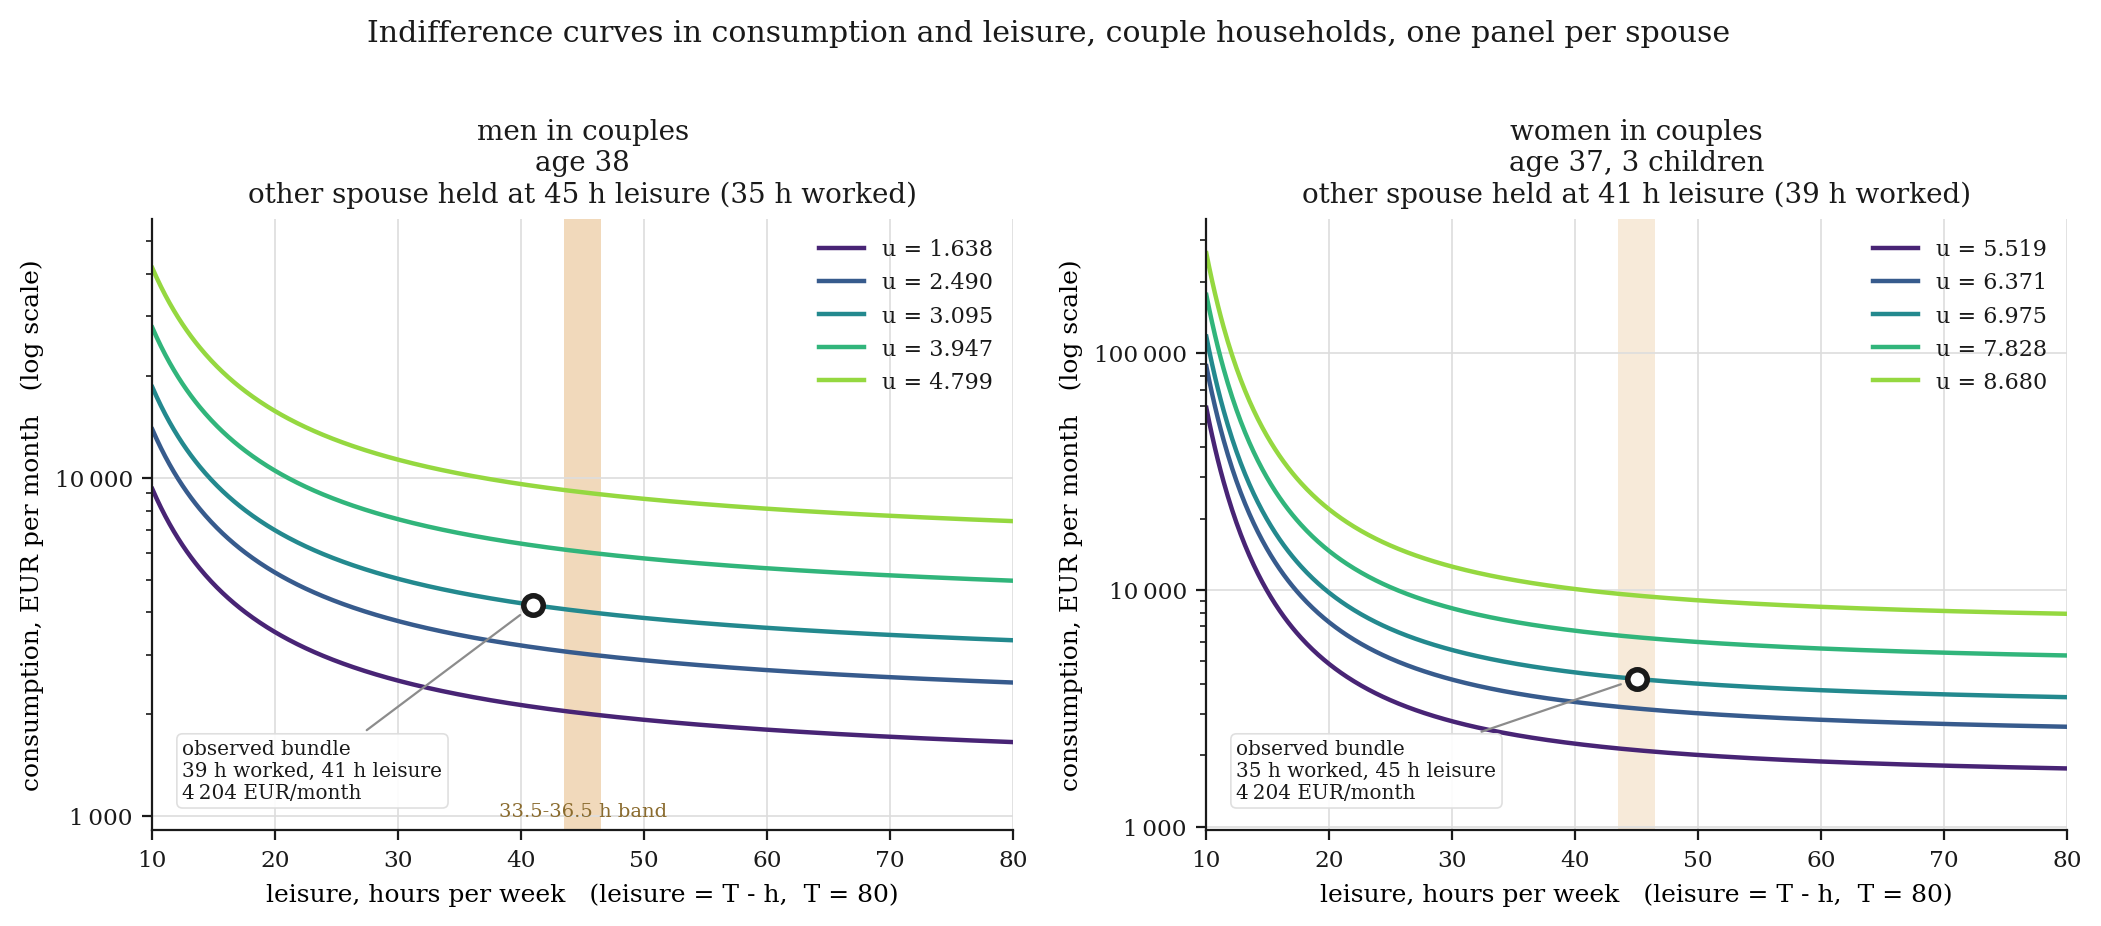
\includegraphics[width=0.95\linewidth,height=\textheight,keepaspectratio,alt={Indifference curves in consumption and joint leisure, couple households. Population: one representative couple household, the medoid on the same criteria, with the partner's leisure held at its observed value. Units: leisure in hours per week per spouse, consumption in euros per month. Status: model-implied preference object at the estimated parameters; conditional slices, not attainable sets.}]{figures/v3/figP02_indifference_curves_couples.png}
\caption{Indifference curves in consumption and joint leisure, couple households. Population: one representative couple household, the medoid on the same criteria, with the partner's leisure held at its observed value. Units: leisure in hours per week per spouse, consumption in euros per month. Status: model-implied preference object at the estimated parameters; conditional slices, not attainable sets.}
\end{figure}

The couples counterpart, with the partner's leisure held at its observed value. These are conditional slices: the joint object is a surface, and reading two slices as if they were one household's trade-off would be wrong.

\begin{figure}
\centering
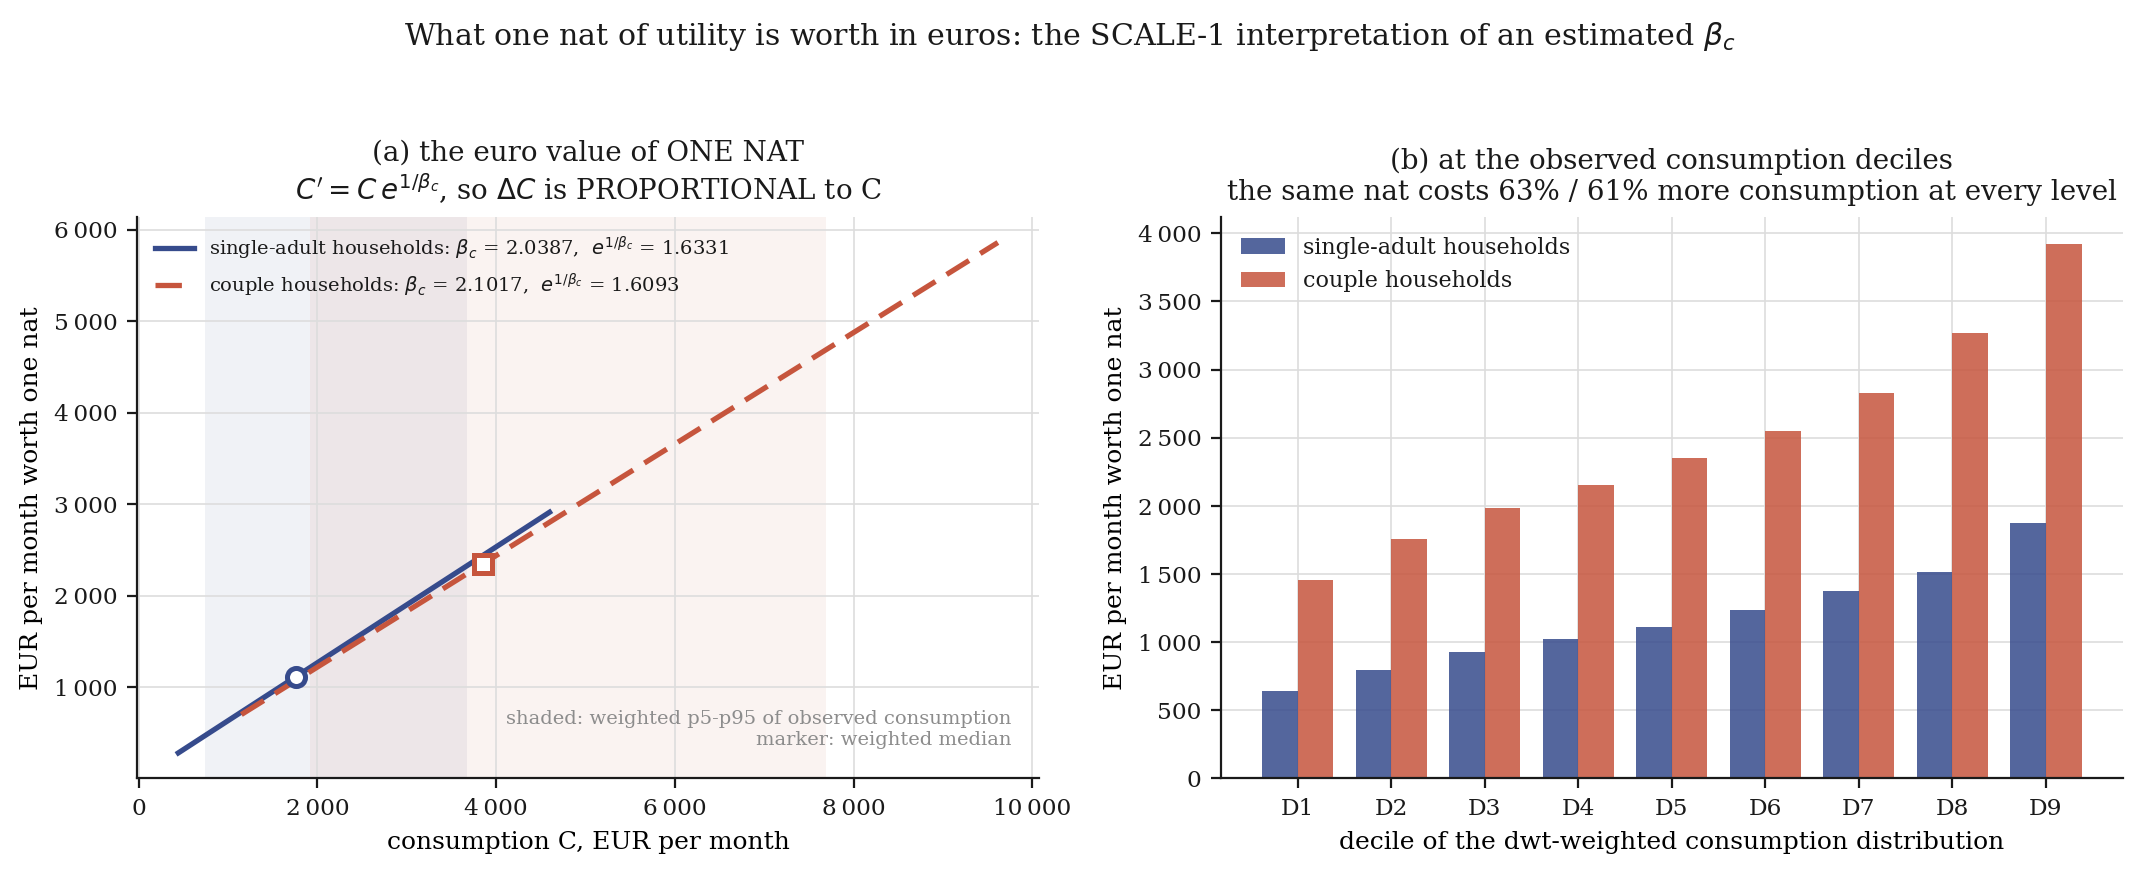
\includegraphics[width=0.95\linewidth,height=\textheight,keepaspectratio,alt={The euro value of one nat of utility under log consumption. Population: the representative households of each block, evaluated across the supported consumption range. Units: euros of monthly disposable consumption per nat of utility; a nat is the natural unit of the unit-scale index. Status: model-implied at the estimated consumption weight. The value is proportional rather than fixed, so it rises with the consumption at which it is evaluated and has no single euro figure independent of a baseline.}]{figures/v3/figP05_euro_value_of_one_nat.png}
\caption{The euro value of one nat of utility under log consumption. Population: the representative households of each block, evaluated across the supported consumption range. Units: euros of monthly disposable consumption per nat of utility; a nat is the natural unit of the unit-scale index. Status: model-implied at the estimated consumption weight. The value is proportional rather than fixed, so it rises with the consumption at which it is evaluated and has no single euro figure independent of a baseline.}
\end{figure}

What one nat of utility is worth in euros. Because consumption enters in logs, a nat is a \emph{proportional} change: it multiplies consumption by a fixed factor, so its euro value rises with the consumption at which it is evaluated and there is no single euro figure that describes it. The panel draws that dependence across the supported range, which is why every euro statement about the shock scale in this document is quoted against a named baseline consumption.

\begin{figure}
\centering
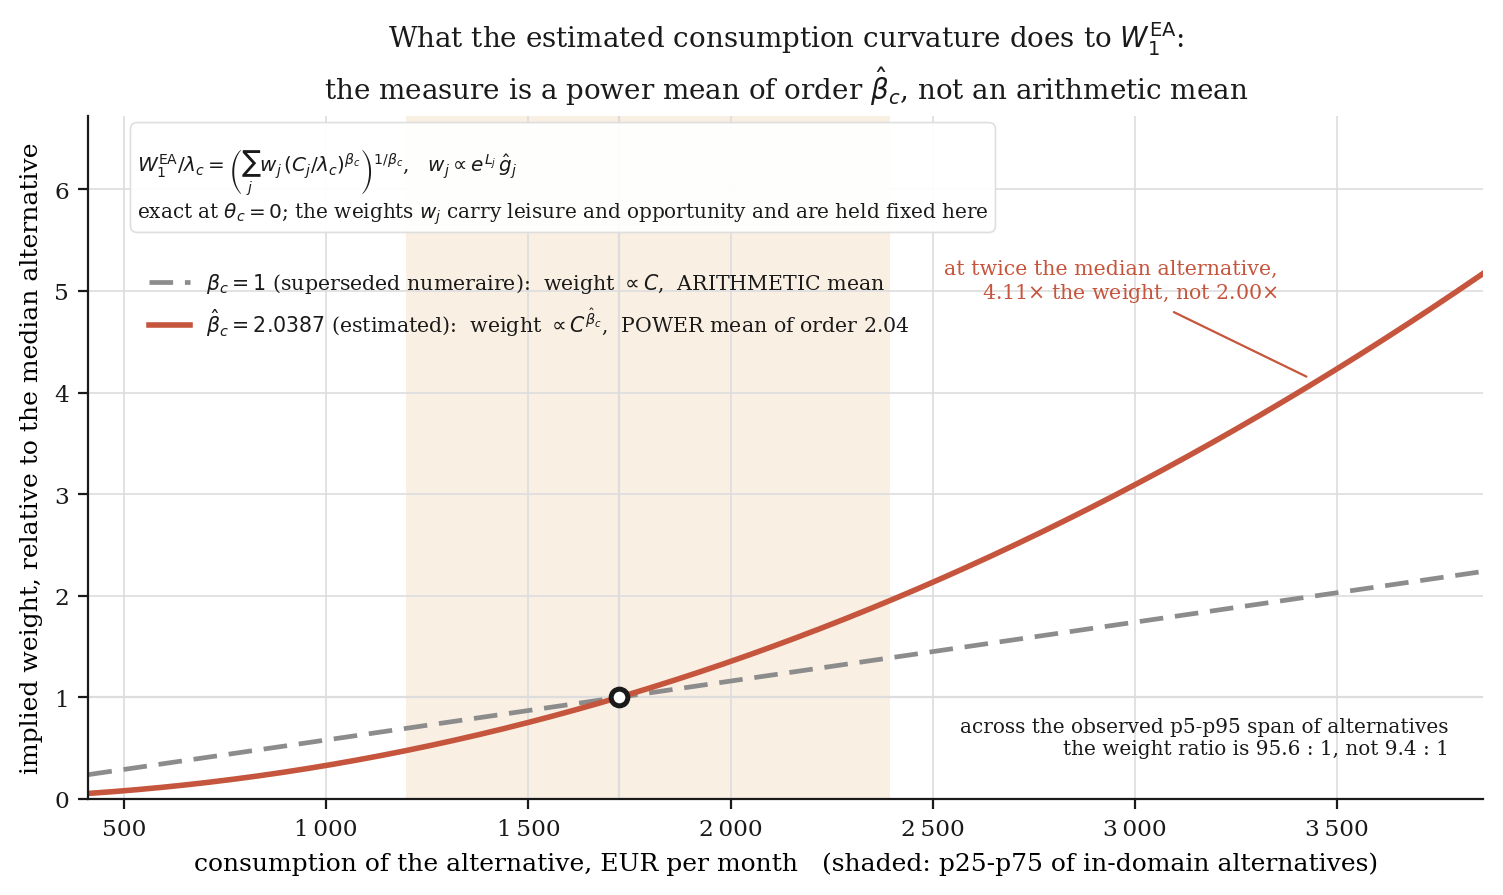
\includegraphics[width=0.95\linewidth,height=\textheight,keepaspectratio,alt={The power-mean weighting of the money metric: the implied weight on an alternative as a function of its consumption. Population: the alternatives of the corrected single-adult frame. Units: horizontal axis euros of monthly disposable consumption; vertical axis a dimensionless relative weight, one at the median alternative. Status: model-implied at the estimated consumption weight. At an order above one the curve rises with consumption, which is the sense in which the measure weights well-paid reachable packages more heavily than an arithmetic mean would.}]{figures/v3/figP07_w1_power_mean_weighting.png}
\caption{The power-mean weighting of the money metric: the implied weight on an alternative as a function of its consumption. Population: the alternatives of the corrected single-adult frame. Units: horizontal axis euros of monthly disposable consumption; vertical axis a dimensionless relative weight, one at the median alternative. Status: model-implied at the estimated consumption weight. At an order above one the curve rises with consumption, which is the sense in which the measure weights well-paid reachable packages more heavily than an arithmetic mean would.}
\end{figure}

Finally, the weighting the money metric actually applies. The welfare section shows that the measure is a power mean of order equal to the estimated consumption weight, and this panel draws what that means for a single alternative: the implied weight as a function of the consumption attached to it, normalized to one at the median alternative. Because the estimated order is above one the curve rises, so a household's well-paid reachable packages count for more than they would under simple averaging. At an order of one the curve would be flat and the mean arithmetic; the flat case is a restriction, and the data reject it.

\bibliographystyle{plainnat}
\bibliography{JMP_working_paper_for_seminar_v4}
\end{document}
